\documentclass[aps,superscriptaddress,floatfix,nofootinbib,showpacs,amsmath,amssymb,altaffilletter,floatfix,onecolumn]{revtex4-1}
%add "rmp" within document class to make it double column and "twocolumn"
%---

%--- Packages
\usepackage[colorlinks=true,pdfstartview=FitV,linkcolor=blue,citecolor=blue,urlcolor=blue]{hyperref}
\usepackage[separate-uncertainty,retain-explicit-plus,per-mode=symbol,binary-units]{siunitx}
\usepackage{array,mathtools,amssymb,dcolumn}
\usepackage{amsmath}
\usepackage[below]{placeins}
\usepackage[table]{xcolor}
\usepackage{tikz}
\usepackage{afterpage}
\usepackage{lineno}
\usepackage{paralist}
\usepackage{listings}
\usepackage{array}
\usepackage[version=4]{mhchem}
\usepackage{multirow}
\usepackage{eurosym}
\usepackage{pagecolor}
\usepackage{fancyhdr}
%--- 1 inch margins
\usepackage{calc}
\setlength\textwidth{6.5in}
\setlength\textheight{9in}
\setlength\oddsidemargin{(\paperwidth-\textwidth)/2 - 1in} 
\setlength\evensidemargin{(\paperwidth-\textwidth)/2 - 1in} 
\setlength\topmargin{(\paperheight-\textheight-\headheight-\headsep-\footskip)/2 - 1in}
%--- Language
\lstset{language=C++,basicstyle=\ttfamily}
%--- Floats Placement
\setlength\textfloatsep{5pt}
\setlength\abovecaptionskip{5pt}
%--- Counters
\newcounter{mylistcounter}
%--- Text and References
\newcommand{\myrefs}[2]{\href{http://dx.doi.org/#2}{#1}}
\newcommand{\mref}[1]{\href{http://#1}{#1}}
\newcommand{\elog}[1]{\href{https://blackhole.lngs.infn.it/DS-50kg/#1}{#1}}
\newcommand{\mrefsec}[1]{\href{https://#1}{#1}}
\newcommand{\mrefs}[2]{\href{http://#2}{#1}}
\newcommand{\arxiv}[1]{\href{http://arxiv.org/abs/#1}{arxiv:#1}}
\newcommand{\grant}[2]{#1-#2}
\newcommand{\docdb}[1]{\href{http://darkside-docdb.fnal.gov:8080/cgi-bin/ShowDocument?docid=#1}{DarkSide DocDB \##1}}
\newcommand{\cmt}[2]{\indent{\tt \color{blue}#1: \color{red}#2}}
\newcommand{\chk}[1]{{\tt \color{red}To be checked:~#1}}
\newcommand{\fchk}[1]{{\tt \color{red}Figure to be replaced:~#1}}
\newcommand{\event}[2]{{\tt Event\# #1, Run\# #2}}
\newcommand{\minitab}[3]{\begin{tabular}{@{}#1@{}}{#2}\\{#3}\end{tabular}}
%--- Software Packages
\newcommand{\FLUKA}{\mbox{FLUKA}}
\newcommand{\Geant}{\mbox{Geant4}}
\newcommand{\GFDS}{\mbox{G4DS}}
\newcommand{\SOURCES}{\mbox{SOURCES4A}}
\newcommand{\TALYS}{\mbox{TALYS}}
\newcommand{\SRIM}{\mbox{SRIM}}
\newcommand{\LabVIEW}{\mbox{NI LabVIEW}}
\newcommand{\CERNRoot}{\mbox{Root}}
%--- Functions
\newcommand{\logten}{\ensuremath{\log_{10}}}
%--- Units
\DeclareSIUnit\c{\mbox{$c$}}
\DeclareSIUnit\magn{\mbox{$\times$}}
\DeclareSIUnit\min{min}
\DeclareSIUnit\week{week}
\DeclareSIUnit\year{yr}
\DeclareSIUnit\years{years}
\DeclareSIUnit\yr{yr}
\DeclareSIUnit\standard{std}
\DeclareSIUnit\str{sr}
\DeclareSIUnit\ppm{ppm}
\DeclareSIUnit\ppb{ppb}
\DeclareSIUnit\ppt{ppt}
\DeclareSIUnit\pe{PE}
\DeclareSIUnit\spe{SPE}
\DeclareSIUnit\ev{events}
\DeclareSIUnit\ct{counts}
\DeclareSIUnit\neutron{\mbox{$n$}}
\DeclareSIUnit\smp{samples}
\DeclareSIUnit\Sample{S}
\DeclareSIUnit\ch{ch}
\DeclareSIUnit\hit{hit}
\DeclareSIUnit\hits{hits}
\DeclareSIUnit\bin{(\mbox{5-PE}~bin)}
\DeclareSIUnit\sgm{\mbox{$\sigma$}}
\DeclareSIUnit\rms{RMS}
\DeclareSIUnit\keVr{\mbox{keV$_{\rm nr}$}}
\DeclareSIUnit\keVee{\mbox{keV$_{e{\rm e}}$}}
\DeclareSIUnit\ph{photons}
\DeclareSIUnit\pm{PMT}
\DeclareSIUnit\inch{''}
\DeclareSIUnit\bit{bit}
\DeclareSIUnit\sample{samples}
\DeclareSIUnit\barn{barn}
\DeclareSIUnit\bara{bar}
\DeclareSIUnit\barg{barg}
\DeclareSIUnit\mlardepth{\mbox(meter~of~\LAr~depth)}
\DeclareSIUnit\Curie{Ci}
\DeclareSIUnit\psi{psi}
\DeclareSIUnit\parsec{pc}
\DeclareSIUnit\liveday{\mbox{live-days}}
\DeclareSIUnit\days{\mbox{days}}
\DeclareSIUnit\day{\mbox{day}}
\DeclareSIUnit\miles{\mbox{miles}}
\DeclareSIUnit\degreeC{\mbox{$^{\circ}$C}}
\DeclareSIUnit\electron{\mbox{$e^-$}}
\DeclareSIUnit\Euro{\mbox{\euro}}
\DeclareSIUnit\cph{cph}
\DeclareSIUnit\neq{neq}
%--- Energies, Branching Ratios, and Abundances
\newcommand{\BR}{\mbox{BR}}
\newcommand{\EC}{\mbox{EC}}
\newcommand{\PositronAnnihilationGammaEnergy}{\SI{511}{\keV}}
\newcommand{\PbXRayEnergy}{\SI{46}{\keV}}
\newcommand{\HOneNeutronCaptureGammaEnergy}{\SI{2.2}{\MeV}}
\newcommand{\LiSixNaturalAbundance}{\SI{7.5}{\percent}}
\newcommand{\LiSixNeutronCaptureCrossSection}{\SI{941}{\barn}}
\newcommand{\LiSixNeutronCaptureTritonEnergy}{\SI{2.73}{\MeV}}
\newcommand{\LiSixNeutronCaptureAlphaEnergy}{\SI{2.05}{\MeV}}
\newcommand{\LiSixNeutronCaptureTritonAlphaQuenchedEnergy}{\SIrange[range-units=single]{400}{500}{\keVee}}
\newcommand{\BTenNaturalAbundance}{\SI{20}{\percent}}
\newcommand{\BTenNeutronCaptureCrossSection}{\SI{3840}{\barn}}
\newcommand{\BTenNeutronCaptureGroundDecayBR}{\SI{6.4}{\percent}}
\newcommand{\BTenNeutronCaptureGroundDecayAlphaEnergy}{\SI{1775}{\keV}}
\newcommand{\BTenNeutronCaptureExcitedDecayBR}{\SI{93.6}{\percent}}
\newcommand{\BTenNeutronCaptureExcitedDecayGammaEnergy}{\SI{478}{\keV}}
\newcommand{\BTenNeutronCaptureExcitedDecayAlphaEnergy}{\SI{1471}{\keV}}
\newcommand{\BTenNeutronCaptureExcitedDecayAlphaQuenchedEnergy}{\SIrange[range-units=single]{30}{35}{\keVee}}
\newcommand{\BTenNeutronCaptureExcitedDecayAlphaPE}{\SIrange[range-units=single]{25}{35}{\pe}}
\newcommand{\COneFourQValue}{\SI{156}{\keV}}
\newcommand{\CoFiveSevenQValue}{\SI{122}{\keV}}
\newcommand{\BaOneThreeThreeQValue}{\SI{356}{\keV}}
\newcommand{\CsOneThreeSevenQValue}{\SI{662}{\keV}}
\newcommand{\ArThreeSevenDecay}{\EC}
\newcommand{\ArThreeSevenBR}{\SI{100}{\percent}}
\newcommand{\ArThreeSevenQValue}{\SI{2.7}{\keV}}
\newcommand{\ArThreeSevenMeanLife}{\SI{50.51(3)}{\day}}
\newcommand{\ArThreeSevenHalfLife}{\SI{35.04}{\day}}
\newcommand{\ArThreeSevenKOneBR}{\SI{81.5}{\percent}}
\newcommand{\ArThreeSevenKTwoToFourBR}{\SI{8.7}{\percent}}
\newcommand{\ArThreeSevenKCaptureXRaysEnergy}{\SI{2.82}{\keV}}
\newcommand{\ArThreeNineQValue}{\SI{565}{\keV}}
\newcommand{\ArThreeNineMeanLife}{\SI{388}{\year}}
\newcommand{\RbEightThreeMeanLife}{\SI{124.4}{\day}}
\newcommand{\RbEightFiveMGammaEnergy}{\SI{514}{\keV}}
\newcommand{\RbEightFiveMMeanLife}{\SI{1.464}{\micro\s}}
\newcommand{\KrEightThreeQValue}{\SI{41.5}{\keV}}
\newcommand{\KrEightThreeMOneMeanLife}{\SI{2.64}{\hour}}
\newcommand{\KrEightThreeMOneECEnergy}{\SI{32.1}{\keV}}
\newcommand{\KrEightThreeMTwoMeanLife}{\SI{222}{\nano\second}}
\newcommand{\KrEightThreeMTwoECEnergy}{\SI{9.4}{\keV}}
\newcommand{\KrEightThreeMOneTwoECEnergy}{\SI{41.5}{\keV}}
\newcommand{\KrEightFiveGroundDecayQValue}{\SI{687}{\keV}}
\newcommand{\KrEightFiveExcitedDecayBR}{\SI{0.43}{\percent}}
\newcommand{\KrEightFiveExcitedDecayQValue}{\SI{173}{\keV}}
\newcommand{\GdNatNeutronCaptureCrossSection}{\SI{48890}{\barn}}
\newcommand{\PbTwoOneZeroHalfLife}{\SI{22.3}{\yr}}
\newcommand{\PbTwoOneZeroMeanLife}{\SI{32.0}{\yr}}
\newcommand{\PoTwoOneZeroAlphaEnergy}{\SI{5.3}{\MeV}}
\newcommand{\PoTwoOneTwoAlphaEnergy}{\SI{8.78}{\MeV}}
\newcommand{\BiTwoOneTwoAlphaOneEnergy}{\SI{6.09}{\MeV}}
\newcommand{\BiTwoOneTwoAlphaTwoEnergy}{\SI{6.05}{\MeV}}
\newcommand{\BiTwoOneTwoHalfLife}{\SI{10.6}{\hour}}
\newcommand{\PoTwoOneSixAlphaEnergy}{\SI{6.78}{\MeV}}
\newcommand{\RnTwoTwoZeroHalfLife}{\SI{56}{\second}}
\newcommand{\RnTwoTwoZeroAlphaEnergy}{\SI{6.29}{\MeV}}
\newcommand{\RnTwoTwoTwoHalfLife}{\SI{3.8}{\day}}
\newcommand{\RaTwoTwoFourHalfLife}{\SI{3.6}{\day}}
\newcommand{\ThTwoTwoEightHalfLife}{\SI{1.9}{\yr}}
\newcommand{\AmTwoFourGammaOneEnergy}{\SI{59.5}{\keV}}
\newcommand{\AmTwoFourOneGammaTwoBR}{\SI{56}{\percent}}
\newcommand{\AmBeGammaEnergy}{\SI{4.4}{\MeV}}
\newcommand{\AmBe}{\ce{^241AmBe}}
\newcommand{\AmC}{\ce{^241Am^13C}}
\newcommand{\AmCNeutronEnergy}{\SI{4}{\MeV}}
\newcommand{\DD}{\ce{^2D}-\ce{^2D}}
\newcommand{\DDNeutronEnergy}{\SI{2.45}{\MeV}}
\newcommand{\AArArThreeNineOverArFourZeroRatio}{\num{8E-16}}
\newcommand{\AArArThreeNineActivity}{\SI{1}{\becquerel\per\kg}}
\newcommand{\NeutronsPerChainDecayUTh}{\numrange{E-5}{E-7}}
\newcommand{\LArRadiogenicNeutronInteractionLength}{\SI{~10}{\cm}}
%--- Cosmology
\newcommand{\LCDM}{\mbox{$\Lambda$CDM}}
%--- Solar Neutrinos
\newcommand{\PP}{\mbox{$pp$}}
\newcommand{\PEP}{\mbox{$pep$}}
\newcommand{\CNO}{\mbox{CNO}}
%--- Names
\newcommand{\DS}{\mbox{DarkSide}}
\newcommand{\DSt}{\mbox{DarkSide-10}}
\newcommand{\DSf}{\mbox{DarkSide-50}}
\newcommand{\DSp}{\mbox{DarkSide-Proto}}
\newcommand{\DSk}{\mbox{DarkSide-20k}}
\newcommand{\DSs}{\mbox{DS}}
\newcommand{\DSts}{\mbox{DS-10}}
\newcommand{\DSfs}{\mbox{DS-50}}
\newcommand{\DSps}{\mbox{DS-Proto}}
\newcommand{\DSks}{\mbox{DS-20k}}
\newcommand{\DSCollaborators}{\num{\sim~300}}
\newcommand{\DSInstitutes}{\num{\sim~70}}
\newcommand{\DSCountries}{\num{15}}
\newcommand{\GADMC}{\mbox{GADMC}}
\newcommand{\DEAP}{\mbox{DEAP-3600}}
\newcommand{\mCLEAN}{\mbox{MiniCLEAN}}
\newcommand{\ArDM}{\mbox{ArDM}}
\newcommand{\Argo}{\mbox{Argo}}
\newcommand{\ThreeDPi}{\mbox{3D$\pi$}}
\newcommand{\FBP}{\mbox{FBP}}
\newcommand{\BX}{\mbox{Borexino}}
\newcommand{\SNO}{\mbox{SNO}}
\newcommand{\SCENE}{\mbox{SCENE}}
\newcommand{\ReD}{\mbox{ReD}}
\newcommand{\ARIS}{\mbox{ARIS}}
\newcommand{\Urania}{\mbox{Urania}}
\newcommand{\Aria}{\mbox{Aria}}
\newcommand{\Seruci}{\mbox{Seruci}}
\newcommand{\SeruciZero}{\mbox{Seruci-0}}
\newcommand{\SeruciOne}{\mbox{Seruci-I}}
\newcommand{\SeruciTwo}{\mbox{Seruci-II}}
\newcommand{\LOGAN}{\mbox{LOGAN}}
\newcommand{\DART}{\mbox{DART}}
\newcommand{\MAWG}{M\&A\,WG}
\newcommand{\CTF}{\mbox{CTF}}
\newcommand{\WBS}{\mbox{WBS}}
\newcommand{\CROne}{\mbox{CR1}}
\newcommand{\CRH}{\mbox{CRH}}
\newcommand{\LSV}{\mbox{LSV}}
\newcommand{\WCV}{\mbox{WCV}}
\newcommand{\wt}{\mbox{WT}}
\newcommand{\TPC}{\mbox{TPC}}
\newcommand{\TPCs}{\mbox{TPCs}}
\newcommand{\LArTPC}{\mbox{LAr~TPC}}
\newcommand{\LArTPCs}{\mbox{LAr~TPCs}}
\newcommand{\calis}{\mbox{CALIS}}
\newcommand{\UV}{\mbox{UV}}
\newcommand{\NUV}{\mbox{NUV}}
\newcommand{\TMF}{\mbox{TMF}}
\newcommand{\PMT}{\mbox{PMT}}
\newcommand{\PMTs}{\mbox{\PMT s}}
\newcommand{\MCP}{\mbox{MCP}}
\newcommand{\MCPPMT}{\mbox{\MCP-\PMT}}
\newcommand{\MCPPMTs}{\mbox{\MCPPMT s}}
\newcommand{\SiPM}{\mbox{SiPM}}
\newcommand{\SiPMs}{\mbox{SiPMs}}
\newcommand{\RGBHd}{\mbox{RGB-HD}}
\newcommand{\RGBHdSf}{\mbox{RGB-HD-SF}}
\newcommand{\RGBHdSfHRq}{\mbox{RGB-HD-HR$_q$}}
\newcommand{\RGBHdSfLRq}{\mbox{RGB-HD-LR$_q$}}
\newcommand{\NUVHd}{\mbox{NUV-HD}}
\newcommand{\NUVHdSf}{\mbox{NUV-HD-SF}}
\newcommand{\NUVHdLf}{\mbox{NUV-HD-LF}}
\newcommand{\NUVHdSfHRq}{\mbox{NUV-HD-SF-HR$_q$}}
\newcommand{\NUVHdSfLRq}{\mbox{NUV-HD-SF-LR$_q$}}
\newcommand{\NUVHdLfHRq}{\mbox{NUV-HD-LF-HR$_q$}}
\newcommand{\NUVHdLfLRq}{\mbox{NUV-HD-LF-LR$_q$}}
\newcommand{\HRq}{\mbox{HR$_q$}}
\newcommand{\LRq}{\mbox{LR$_q$}}
\newcommand{\HD}{\mbox{HD}}
\newcommand{\CTE}{\mbox{CTE}}
\newcommand{\PCB}{\mbox{PCB}}
\newcommand{\PCBs}{\mbox{PCBs}}
\newcommand{\TSV}{\mbox{TSV}}
\newcommand{\TSVs}{\mbox{TSVs}}
\newcommand{\tile}{\mbox{tile}}
\newcommand{\tiles}{\mbox{tiles}}
\newcommand{\SPAD}{\mbox{SPAD}}
\newcommand{\SPADs}{\mbox{SPADs}}
\newcommand{\QE}{\mbox{QE}}
\newcommand{\PDE}{\mbox{PDE}}
\newcommand{\OV}{\mbox{OV}}
\newcommand{\LV}{\mbox{LV}}
\newcommand{\SCR}{\mbox{SCR}}
\newcommand{\DCR}{\mbox{DCR}}
\newcommand{\DiCT}{\mbox{DiCT}}
\newcommand{\DeCT}{\mbox{DeCT}}
\newcommand{\AP}{\mbox{AP}}
\newcommand{\DLED}{\mbox{DLED}}
\newcommand{\TCNR}{\mbox{TCNR}}
\newcommand{\TCNP}{\mbox{TCNP}}
\newcommand{\CMOS}{\mbox{CMOS}}
\newcommand{\HLST}{\mbox{HLST}}
\newcommand{\SQB}{\mbox{SQB}}
\newcommand{\SQBs}{\mbox{\SQB s}}
\newcommand{\TRB}{\mbox{TRB}}
\newcommand{\TRBs}{\mbox{\TRB s}}
\newcommand{\WIMP}{\mbox{WIMP}}
\newcommand{\WIMPs}{\mbox{\WIMP s}}
\newcommand{\MC}{\mbox{MC}}
\newcommand{\DAQ}{\mbox{DAQ}}
\newcommand{\ADC}{\mbox{ADC}}
\newcommand{\ADCs}{\mbox{\ADC s}}
\newcommand{\TDC}{\mbox{TDC}}
\newcommand{\TDCs}{\mbox{\TDC s}}
\newcommand{\artdaq}{\mbox{artdaq}}
\newcommand{\TMB}{\mbox{TMB}}
\newcommand{\PC}{\mbox{PC}}
\newcommand{\PCTMB}{\mbox{\PC-\TMB}}
\newcommand{\PPO}{\mbox{PPO}}
\newcommand{\BisMSB}{\mbox{BisMSB}}
\newcommand{\POPOP}{\mbox{POPOP}}
\newcommand{\DIN}{\mbox{DIN}}
\newcommand{\LAB}{\mbox{LAB}}
\newcommand{\PXE}{\mbox{PXE}}
\newcommand{\ITO}{\mbox{ITO}}
\newcommand{\PTFE}{\mbox{PTFE}}
\newcommand{\FEP}{\mbox{FEP}}
\newcommand{\TPB}{\mbox{TPB}}
\newcommand{\og}{\mbox{Operations Group}}
\newcommand{\VUV}{\mbox{VUV}}
\newcommand{\LAr}{\ce{LAr}}
\newcommand{\GAr}{\ce{GAr}}
\newcommand{\AAr}{\ce{AAr}}
\newcommand{\UAr}{\ce{UAr}}
\newcommand{\DAr}{\ce{DAr}}
\newcommand{\LRAr}{\ce{LRAr}}
\newcommand{\LIN}{\ce{LN2}}
\newcommand{\LXe}{\ce{LXe}}
\newcommand{\HPGe}{\mbox{HPGe}}
\newcommand{\HVFT}{\mbox{HVFT}}
\newcommand{\UHMWPE}{\mbox{UHMWPE}}
\newcommand{\TOF}{\mbox{TOF}}
\newcommand{\PET}{\mbox{PET}}
\newcommand{\TOFPET}{\mbox{\TOF-\PET}}
\newcommand{\PETCT}{\mbox{\PET /CT}}
\newcommand{\FDG}{\mbox{\ce{^18F}-FDG}}
\newcommand{\LOR}{\mbox{LOR}}
\newcommand{\CPU}{\mbox{CPU}}
\newcommand{\CT}{\mbox{CT}}
\newcommand{\CPUs}{\mbox{CPUs}}
\newcommand{\STEM}{\mbox{STEM}}
\newcommand{\ROI}{\mbox{ROI}}
\newcommand{\SPE}{\mbox{SPE}}
\newcommand{\SNR}{\mbox{SNR}}
\newcommand{\SNRAmp}{\mbox{SNR$_{\rm Amplitude}$}}
\newcommand{\SNRCharge}{\mbox{SNR$_{\rm Charge}$}}
\newcommand{\SNRFast}{\mbox{SNR$_{\rm Fast}$}}
\newcommand{\SNRFilter}{\mbox{SNR$_{\rm Filtered}$}}
\newcommand{\OA}{\mbox{OA}}
\newcommand{\GBP}{\mbox{GBP}}
\newcommand{\TIA}{\mbox{TIA}}
\newcommand{\TIAs}{\mbox{\TIA s}}
\newcommand{\FEB}{\mbox{FEB}}
\newcommand{\FEBs}{\mbox{\FEB s}}
\newcommand{\VFEB}{\mbox{VFEB}}
\newcommand{\VFEBs}{\mbox{\VFEB s}}
\newcommand{\VDCB}{\mbox{VDCB}}
\newcommand{\VDCBs}{\mbox{\VDCB s}}
\newcommand{\AVol}{\mbox{$A_{\tiny\rm Vol}$}}
\newcommand{\NoG}{\mbox{NG}}
\newcommand{\NoGTrue}{\mbox{$\NoG_{\rm True}$}}
\newcommand{\Tz}{\mbox{$T_z$}}
\newcommand{\eno}{\mbox{$e_n$}}
\newcommand{\enot}{\mbox{$e_n^2$}}
\newcommand{\ino}{\mbox{$i_n$}}
\newcommand{\inot}{\mbox{$i_n^2$}}
\newcommand{\Vno}{\mbox{$V_n$}}
\newcommand{\Vnot}{\mbox{$V_n^2$}}
\newcommand{\VnoTot}{\mbox{$V_n^{\rm Tot}$}}
\newcommand{\fRes}{\mbox{$f_{\rm Res}$}}
\newcommand{\FTDb}{\mbox{$f_{\rm 3Db}$}}
\newcommand{\FSDb}{\mbox{$f_{\rm 6Db}$}}
\newcommand{\TDb}{\SI{3}{\decibel}}
\newcommand{\SDb}{\SI{6}{\decibel}}
\newcommand{\PSDno}{\mbox{$\rm PSD_{n}$}}
\newcommand{\PSDnoReferencePower}{\SI{1}{\milli\watt}}
\newcommand{\NSF}{\mbox{NSF}}
\newcommand{\RAS}{\mbox{RAS}}
\newcommand{\GSSI}{\mbox{GSSI}}
\newcommand{\INFN}{\mbox{INFN}}
\newcommand{\MIUR}{\mbox{MIUR}}
\newcommand{\CERN}{\mbox{CERN}}
\newcommand{\LHC}{\mbox{LHC}}
\newcommand{\CFI}{\mbox{CFI}}
\newcommand{\NSERC}{\mbox{NSERC}}
\newcommand{\LNGS}{\mbox{LNGS}}
\newcommand{\LSC}{\mbox{LSC}}
\newcommand{\SNOLab}{\mbox{SNOLab}}
\newcommand{\TRIUMF}{\mbox{TRIUMF}}
\newcommand{\LNS}{\mbox{LNS}}
\newcommand{\DUNE}{\mbox{DUNE}}
\newcommand{\CNAF}{\mbox{CNAF}}
\newcommand{\PoliMi}{\mbox{PoliMi}}
\newcommand{\FBKTIFPA}{\mbox{FBK/TIFPA}}
\newcommand{\FBK}{\mbox{FBK}}
\newcommand{\MPD}{\mbox{MPD}}
\newcommand{\LFoundry}{\mbox{LFoundry}}
\newcommand{\SensL}{\mbox{SensL}}
\newcommand{\NOA}{\mbox{NOA}}
\newcommand{\LSO}{\mbox{LSO}}
\newcommand{\LYSO}{\mbox{LYSO}}
\newcommand{\CRT}{\mbox{CRT}}
\newcommand{\ASIC}{\mbox{ASIC}}
\newcommand{\ASICs}{\mbox{ASICs}}
\newcommand{\PSA}{\mbox{PSA}}
\newcommand{\UHV}{UHV}
\newcommand{\HalfLife}{\mbox{$\tau_{\frac{1}{2}}$}}
\newcommand{\ICPMS}{\mbox{ICP-MS}}
\newcommand{\LA}{\mbox{LA}}
\newcommand{\LAICPMS}{\mbox{\LA-\ICPMS}}
\newcommand{\BiPo}{\mbox{BiPo-3}}
\newcommand{\PEB}{\mbox{PEB}}
\newcommand{\PEBs}{\mbox{PEBs}}
\newcommand{\VO}{\mbox{VO}}
\newcommand{\LiDaR}{\mbox{LiDaR}}
\newcommand{\ArlonFiveFiveNT}{\mbox{Arlon~55-NT}}
\newcommand{\ArlonEightFiveN}{\mbox{Arlon~85-N}}
\newcommand{\ArlonEightFiveNT}{\mbox{Arlon~85-NT}}
\newcommand{\THERMOUNT}{\mbox{THERMOUNT\textregistered RT\textsuperscript{TM}}}
\newcommand{\Vikuiti}{\mbox{3M Vikuiti\textsuperscript{TM}}}
%--- Global Symbols
\newcommand{\OmegaNonBaryonicFraction}{\num{0.85}}
\newcommand{\OmegaNonBaryonicPercent}{\SI{85}{\percent}}
\newcommand{\RhoDMSymbol}{\mbox{$\rho_{\rm dm}$}}
\newcommand{\RhoDMValue}{\SI{0.3}{\GeV\per\square\c\per\cubic\cm}}
\newcommand{\VelocityNaughtSymbol}{\mbox{$v_0$}}
\newcommand{\VelocityNaughtValue}{\SI{220}{\km\per\s}}
\newcommand{\VelocityEarthSymbol}{\mbox{$v_{\rm Earth}$}}
\newcommand{\VelocityEarthValue}{\SI{232}{\km\per\s}}
\newcommand{\VelocityEscapeSymbol}{\mbox{$v_{\rm escape}$}}
\newcommand{\VelocityEscapeValue}{\SI{544}{\km\per\s}}
\newcommand{\WIMPMassSymbol}{\mbox{m_\chi}}
\newcommand{\WIMPMassLowLimit}{\SI{50}{\GeV\per\square\c}}
\newcommand{\WIMPMassHundredGev}{\SI{100}{\GeV\per\square\c}}
\newcommand{\WIMPMassOneTev}{\SI{1}{\TeV\per\square\c}}
\newcommand{\WIMPMassTenTev}{\SI{10}{\TeV\per\square\c}}
\newcommand{\LArNormalTemperature}{\SI{87}{\kelvin}}
\newcommand{\LINNormalTemperature}{\SI{77}{\kelvin}}
\newcommand{\LXeNormalTemperature}{\SI{165}{\kelvin}}
\newcommand{\RoomTemperature}{\SI{300}{\kelvin}}
\newcommand{\ElectronMass}{\SI{511}{\keV\per\square\c}}
\newcommand{\LHCCenterOfMassEnergy}{\SI{13}{TeV}}
\newcommand{\LHCDirectSearchesWIMPMassTurnoverThreshold}{\text{a few hundred~\si{GeV\per\square\c}}}
\newcommand{\BackgroundFreeRequirement}{\SI{<0.1}{\ev}}
\newcommand{\ZeroBackgroundNinetyPerCentCLEventsLimit}{\SI{2.3}{\ev}}
\newcommand{\NinetyPerCentCL}{\mbox{\SI{90}{\percent}~C.L.}}
\newcommand{\ArScintillationYield}{\SI{4E4}{\ph\per\MeV}}
\newcommand{\ArWaveLength}{\SI{128}{\nano\meter}}
\newcommand{\TPBWaveLength}{\SI{420}{\nano\meter}}
\newcommand{\XeWaveLength}{\SI{172}{\nano\meter}}
\newcommand{\NR}{\mbox{NR}}
\newcommand{\NRs}{\mbox{NRs}}
\newcommand{\ER}{\mbox{ER}}
\newcommand{\ERs}{\mbox{ERs}}
\newcommand{\bg}{\mbox{$\beta/\gamma$}}
\newcommand{\bgs}{\mbox{$\beta/\gamma$'s}}
\newcommand{\gr}{\mbox{$\gamma$-ray}}
\newcommand{\grs}{\mbox{$\gamma$-rays}}
\newcommand{\bta}{\mbox{$\beta$}}
\newcommand{\btas}{\mbox{$\beta$'s}}
\newcommand{\LEff}{\mbox{$\mathcal{L}_{\rm eff}$}}
\newcommand{\SOne}{\mbox{S1}}
\newcommand{\STwo}{\mbox{S2}}
\newcommand{\STwoSoneRatio}{\mbox{S2/S1}}
\newcommand{\SThree}{\mbox{S3}}
\newcommand{\GWL}{\mbox{GWL}}
\newcommand{\LWL}{\mbox{LWL}}
\newcommand{\mbb}{\mbox{$m_{\beta\beta}$}}
\newcommand{\qbb}{\mbox{$Q_{\beta\beta}$}}
\newcommand{\bb}{\mbox{$\beta$$\beta$}}
\newcommand{\obb}{\mbox{0$\nu$$\beta$$\beta$}}
\newcommand{\toh}{\mbox{T$^{0\nu}_{1/2}$}}
\newcommand{\tth}{\mbox{T$^{2\nu}_{1/2}$}}
\newcommand{\aSe}{\mbox{a-\ce{Se}}}

\usepackage{fancyhdr}
\usepackage{array}
\usepackage{enumitem}
\usepackage{graphicx}
\usepackage{wrapfig}
\usepackage[title]{appendix}
\usepackage{float}
%\linespread{0.9}
\fancyhf{}
\renewcommand{\headrulewidth}{0pt}
\rfoot{\thepage}

\headheight 50pt
\newcommand{\hasplogo}{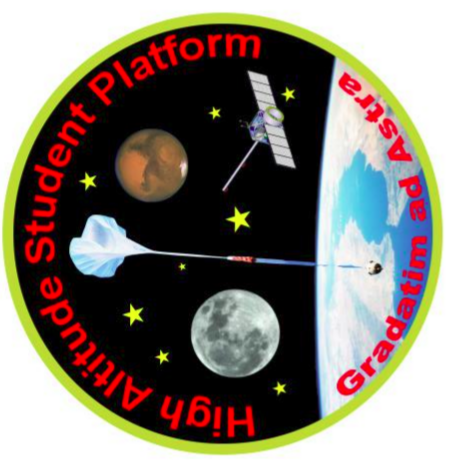
\includegraphics[width=0.08\linewidth]{Figures/logo.pdf}} %Header
\lhead{\hasplogo} %Header
\chead{\vspace*{-2cm}\Large\textbf{HASP Payload Application 2018}} %Header

\pagestyle{fancy}
%\linespread{0}
\renewcommand{\thepage}{}
\renewcommand{\thepage}{\arabic{page}}
\renewcommand\thesection{\arabic{section}}
\renewcommand\thesubsection{\thesection.\arabic{subsection}}
\renewcommand\thesubsubsection{\thesubsection.\arabic{subsubsection}}
\parskip = 6pt %changes spacing between paragraphs
%\nolinenumbers
\makeatletter
\def\p@subsection{}
\makeatother
\makeatletter
\def\p@subsubsection{}
\makeatother
%---
\begin{document}
%---
\title{SORA 2.0: Stratospheric Organism and Radiation Analyzer}

\begin{abstract}
\begin{center}
{\bf Abstract}
\end{center}

The SORA 2.0 payload will again sample for the existence of microorganisms and bacterial spores in the upper atmosphere.  This mission will build upon the first SORA mission in 2017, and help confirm previous findings using a developed captured system. Furthermore, the payload will study different aspects of the surrounding environment such as radiation exposure, temperature, pressure and humidity. The payload has three main scientific objectives. First, build upon and further develop a novel system~\cite{SORA} that will isolate surrounding air and sample for cells. Second, an on-board MiniPIX USB silicon sensor~\cite{silicon_sensor} will analyze exposure to cosmic radiation that microorganisms may encounter. Finally, a mature version of RESU (Realtime Environmental Sensing Unit)~\cite{SORA} will monitor the environmental conditions such as temperature, pressure, and humidity. The payload design will take advantange of additive manufacturing and hobby electronics in its construction to provide an accessible basis for future missions and explore the bounds of the technology available.  

\newpage %Breaks page for the Table of Contents.
\end{abstract}
\newcommand{\Houston}{Department of Physics, University of Houston, Houston, TX 77204, USA}
%--- Add other authors in the order they should appear

\author{S.~A.~Garcia~Morelos}\affiliation{\Houston}
\author{F.~Brooks}\affiliation{\Houston}
\author{S.~Oliver}\affiliation{\Houston}
\author{A.~Walker}\affiliation{\Houston}
\author{K.~Portillo}\affiliation{\Houston}
\author{R.~Masek}\affiliation{\Houston}
\author{D.~Mroczek}\affiliation{\Houston}
\author{D.~De~La~Pena}\affiliation{\Houston}
\author{J.~Juarez}\affiliation{\Houston}
\author{A.~Cruz}\affiliation{\Houston}
\author{D.~Henandez}\affiliation{\Houston}
\author{A.~L.~Renshaw}\affiliation{\Houston}





\setlength{\parindent}{1em}
\setdefaultleftmargin{1em}{1em}{}{}{}{}
%---
\setcounter{page}{0}\thispagestyle{empty}
%---
\maketitle
\onecolumngrid
\setcounter{tocdepth}{2}
\setcounter{page}{0}\thispagestyle{empty}
\tableofcontents
\setcounter{page}{0}\thispagestyle{empty}
\newpage
%---
\onecolumngrid %changed from "twocolumngrid"


%Section: Mission Overview w/ Subsections Mission Statement and Hypotheses
	\section{Mission Statement and Objectives}
\label{sec:Introduction}

Our goal for the HASP 2018 payload is to further build upon the first SORA~\cite{SORA} flight.  In order to confirm our findings from SORA 2017, we need to again collect extremophile bacteria that reside in the upper atmosphere at approximately 36 to 41 kilometers.  A MiniPIX particle detector will be flown onboard to further study the effects of ionizing radiation on these living organisms and other various sensors will gather data pertaining to the environmental conditions in which these extremophiles reside. Due to the limited amount of data for the 20 to 40 kilometer altitude range, we have generated questions, hypotheses and objectives, based on past HASP payloads and other high altitude collection flights, that have thus far remained unanswered or have little corroborating data.

%\begin{figure}[h!]
%  \begin{center}
%    \begin{minipage}[c]{0.45\linewidth}
%      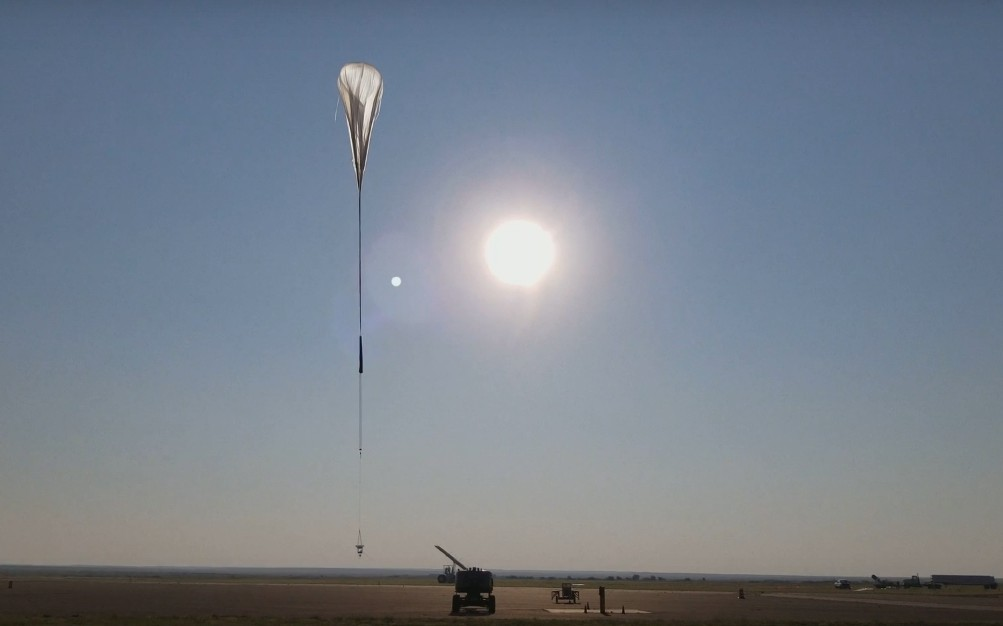
\includegraphics[width=\textwidth]{./Figures/sora_takeoff.jpg}
%      \caption{HASP platform at launch with the SORA payload onboard.}
%      \label{fig:takeoff}
%    \end{minipage}
%    \hfill
%    \begin{minipage}[c]{0.49\linewidth}
%      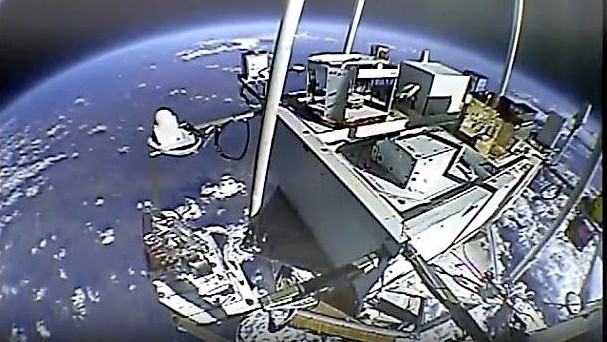
\includegraphics[width=\textwidth]{./Figures/sora_flight.jpg}
%      \caption{HASP platform at float, the SORA payload is the only gold foil covered payload onboard.}
%      \label{fig:float}
%    \end{minipage}
%  \end{center}
%\end{figure}

The main goals for SORA are to collect extremophile organisms that reside in the upper atmosphere, study the effects of surrounding radiation on these organisms in the stratosphere and gather data pertaining to the environmental conditions in which these organisms reside~\cite{SORA}.  More specifically, SORA has two sets of main objectives, along with four additional objectives.

{\bf Primary Scientific Objectives:}
	\begin{enumerate}
	\item Attempt to capture microorganisms in the upper atmosphere at approximately \SIrange{30}{41}{\kilo\meter} of altitude using multiple methods. 
	\item Culture samples and compare the collection medium.
	\item Study the cosmic and terrestrial radiation in which these extremophiles may reside.
	\end{enumerate}
	
{\bf Secondary Scientific Objectives:}
	\begin{enumerate}
	\item Test RESU further and develop a more power-efficient flight control system.
	\item Determine the polar angle of hits on the detector and be able to compare them to payload orientation information.
	\cmt{Andrew W.} {I'm beginning to doubt the usefulness of this aspect as according to Stuart's research on the ISS, measurements of GCRs are isotropic.(Meaning we would probably see very little correleation in terms of polar angle even if it was corrected for payload orientation)}
	\item Further testing of the astrobiology hardware in flight and the methodology for collection of microbes in extreme environments at high-altitude.
	\item Improve pre-and post-flight decontamination procedures.
	\end{enumerate}

\cmt{Andrew W.}{Maybe in terms of science we should focus more on the biological effect of radiation.}

{\bf Engineering Objectives}
	\begin{enumerate}
	\item Implement a variable shutter time for the MiniPIX based on the flux of particles incident on the detector.
	\item Analyze MiniPIX data in real time and downlink relevant radiation statistics.
	\item Implement a redundant data storage mechanism.
	\item Test an improved enclosure against impacts and harsh environments.
	\item Improve astrobiology collection mechanism.
	\end{enumerate}

These goals and objectives are based on the following scientific questions: After confirming that microorganisms are present in the upper atmosphere in our last mission~\ref{SORA}, what extremophiles are present in the upper atmosphere at altitudes of 36 to 41 km?  If extremophiles are captured, can we culture the microorganisms?  What methods are more effective at capturing bacteria for culturing? Finally, with a deeper understanding of the MiniPIX after our first mission, can we collect more data to study cosmic radiation that microoganisms and spores are exposed to on a daily basis? Specifically, can we obtain useful information about the biological effectiveness of this radiation on bacteria through parameters such as linear energy transfer and dose equivalent. \cmt{Andrew R.}{It would be good to revamp or expand on these questions based on the slightly new objectives.}
\cmt{Sam}{I made some changes, I think this would be more fitting.  Andrew W. had a few more ideas for the MiniPIX that we could add}
\cmt{Andrew W.} {Added a more specific MiniPIX scientific goal let me know what you think}

%\begin{itemize}
%	\item Are extremophiles present in the upper atmosphere at altitudes of 36 to 41 km?
%	\item Will the container design protect all components of the data collection system and allow for accurate results?
%	\item Will the Clean Box design prevent sample contamination?
%	\item What are the effects of cosmic and UV radiation to organisms and bacterial spores?
%\end{itemize}

\subsection{Hypothesis and Objectives}
\label{subsec:Hypothesis-Objectives}
\begin{enumerate}
\item Based on the collection results from previous missions such as SORA~\cite{SORA}, we predict the concentration of cells at an altitude of 36 km will be less than 500 cells per liter \citep{LSU}.
	\begin{enumerate}
	\item Objective: Sample a minimum volumetric amount of air at target altitude for the duration of the float phase (approximately 15 to 18 hours).
	%\item Status: This objective was completed in flight, with successful operation of the sampling pump for the duration of the flight, operating at a confirmed current which allowed for air flow through the sample cell for the entire float portion of the mission.  As of November 28th, 2017 the RNA sequencing results from the lab analysis arrived with positive results.  The full interpretation of the results is currently underway as seen in Section~\ref{sec:Astrobiology-Results}.
	\end{enumerate}
\item Based on control samples and testing before flight, we can compare our final flight results to previous applications.
	\begin{enumerate}
	\item Objective: Quantify and characterize any contamination with our laboratory and payload disinfection procedures.
	\item Objective: Minimize the amount of external contamination before flight with thorough decontamination procedures.
	%\item Status: Study is currently underway based on the external lab analysis results which returned RNA sequencing for the collected sample, as well as the control sample.
	\end{enumerate}
%\item Using SolidWorks 3D CAD design software~\cite{Solidworks} and COMSOL Multiphysics Simulation software~\cite{COMSOL}, we can predict what kind of conditions and forces our container will experience.
	%\begin{enumerate}
	%\item Objective: Using results from simulations and real world tests, adapt a structure and a container to ensure the final results are reliable.
	%\item Status: Incomplete - no simulation results.  Main issue was not having enough time to complete in-depth simulations and actual experimental testing proved more reliable.
	%\end{enumerate}
\item Based on measured results of dosage rates, the higher exposure to radiation may change the organism's cellular make-up.
	\begin{enumerate}
	\item Objective: Quantify the intensity and exposure cosmic radiation over the duration of the flight.
	\item Objective: After capturing samples, analyze data and compare biological effects to similar genotypes found on Earth's surface.
	%\item Status: After consultation with biologists at University of Houston (UH), we chose to send the sample for sequencing to see if we captured anything, thus making it hard to compare directly the differences between anything found on Earth and in the atmosphere.  Another mission is necessary to fully complete this objective, but positive results from this mission show the possibilities for a follow-up mission.
	\end{enumerate}
\end{enumerate}

\vspace*{-0.5cm}

	%Scientific Background
		\subsection{Astrobiology}
\label{sec:Astrobiology-Background}

Extremophiles thrive in physically and/or chemically extreme conditions, which are detrimental to most of life on Earth as we know it. These organisms and microbes have been found everywhere, from deep underwater volcano vents to buried ice lakes in Antarctica \cite{Extremophiles}.  As shown in Table~\ref{tab:astrobiotable}, fungi and bacterial spores have previously been found in the stratosphere. Arguably, each successful collection expedition of at least \SI{30}{\kilo\meter} into the upper atmosphere provides information that could be useful in determining what life forms can exist inside and outside of Earth's biosphere. Today, the most common altitude for bacterial collection in the atmosphere occurs in the range of approximately \SIrange{10}{20}{\kilo\meter} above Earth's surface; very little data exists on microbiological samples captured in the stratosphere. Conditions at altitudes of \SIrange{30}{40}{\kilo\meter} are extreme in temperature, pressure and radiation. 

	
%\begin{figure}[H]
%\centering
%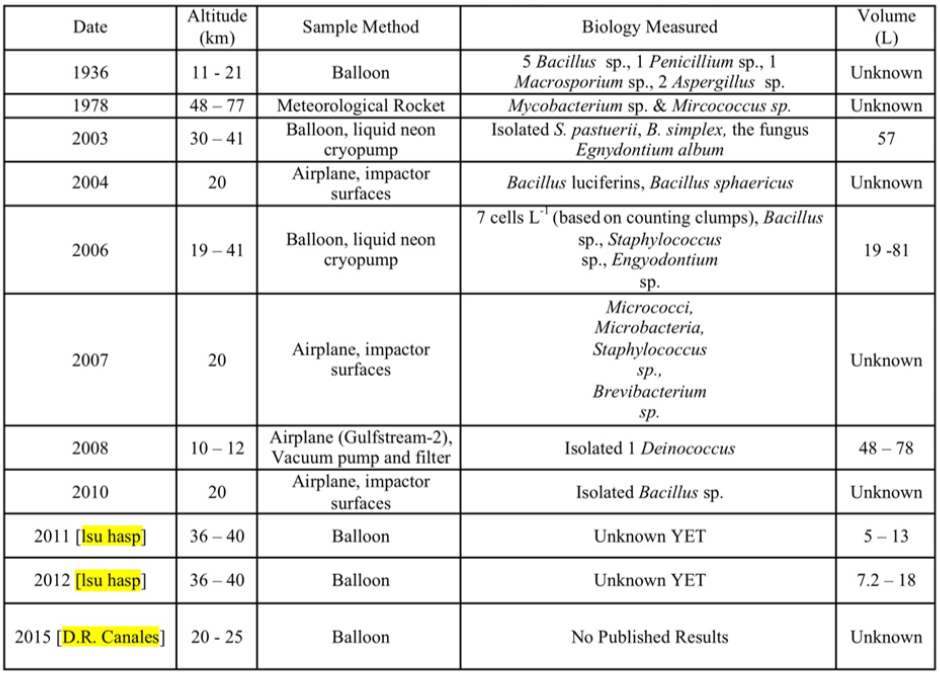
\includegraphics[width=1\textwidth]{./Figures/AstroChart.PNG}
%\caption{}
%\label{fig:AstroHist}
%\end{figure} 




Our experiment is an attempt to further develop our technique for capturing microorganisms in the upper atmosphere, as demonstrated during our 2017~\cite{SORA} flight.  We took inspiration from the LSU HASP 2011, 2012, 2013 flights~\cite{LSU} and from research by D.R. Canales~\cite{canales}.  This flight will also help us further understand our findings from our first flight, and to maybe fully culture these rare microorganisms. We will use two of the KNF N84-4 commercial gas-sampling diaphragm vacuum pumps to sample the air at approximately \SI{33}{\kilo\meter} above Earth's surface. The samples we hope to collect are an important part to expanding our understanding of Earth's biosphere and further studies could provide more insight on how life can be distributed on Earth, and ultimately, through outer-space.

\begin{table}[!ht]
\centering
\caption{History of Microbiological Sampling of the stratosphere~\cite{SORA}.} 
\label{tab:AstroHist} 
\bigskip
\begin{tabular}{|c|c|c|p{6cm}|c|}
\hline
\multicolumn{1}{|c|}{\bfseries Date} & \minitab{c}{\bf Altitude}{\bf (km)} &  \multicolumn{1}{c|}{\bfseries Sample Method} & \multicolumn{1}{p{6cm}|}{\bfseries Biology Measured} & \multicolumn{1}{c|}{\bfseries Volume} \\
\hline
    1936	& 11 - 12 	& Balloon			 			& \minitab{l}{5 Bacillus sp., 1 Penicillium sp.,}{1 Macrosporium sp., 2 Aspergillus sp.} 			& $Unknown$ \\ \hline
    1978	& 48 - 77 	&Meteorological Rocket	 		& Mycobacterium sp., Mircococcus sp.					       							& $Unknown$ 	\\ \hline
    2003	& 30 - 41	& Balloon, liquid neon cryopump	& \minitab{l}{Isolated S. pastuerii, B. simplex,}{the fungus, Egnydontium album}       				& $57$	\\ \hline    
    2004	& 20	 	&Airplane, Impactor Surfaces 	 	& Bacillus luciferins, Bacillus sphaericus			       									& $Unknown$ 	\\ \hline
    2006	& 19 - 41	& Balloon, Liquid Neon Cryopump 	& \minitab{l}{7 cells L-1 (counting clumps), Bacillus sp.,}{Staphylococcus sp., Engyodontium sp.}	& $19-81$ \\ \hline
    2007	& 20	       	& Airplane, Impactor Surfaces 		& \minitab{l}{Micrococci, Microbacteria,}{Staphylococcus sp., Brevibacterium sp.}    				& $Unknown$ \\ \hline
    2010	& 20	       	& Airplane, Impactor Surfaces 		& Isolated Bacillus sp.							     								& $Unknown$\\ \hline
    2017	& 32	       	& Balloon, liquid medium and vacuum pump	&  Multiple findings~\cite{SORA}							     								& $Unknown$\\ \hline
\end{tabular}
\label{tab:astrobiotable}
\medskip
\end{table}

		\subsection{Radiation Introduction}
\label{sec: Radiation Background}

\subsubsection{Cosmic Radiation}
The study of the biological effects of cosmic radiation in space or near space environments is important for human space travel. Long term space travel necessarily requires humans and other biological specimens to be exposed to high levels of radiation for extended periods of time, so understanding the amount the of radiation exposure experienced from galactic cosmic rays (GCRs) has important applications for flights to Mars and beyond. Also, the understanding of cosmic rays specifically in Earth's atmosphere has important applications to commercial airplane flights as they generally operate at an altitude with far higher levels of radiation exposure than at the surface of Earth. 

Our goals for the radiation portion of our payload are two fold, to measure radiation levels at various layers in the atmosphere to determine its possible effects on microorganisms, and to use a MiniPIX particle detector in the extreme environment of the stratosphere to gather data regarding GCRs. Using the results from the previous iteration of SORA~\cite{SORA} as a baseline, we know the capabilites of the MiniPIX, and we will make several design changes to improve the efficiency of our system and to produce more in-depth data analysis. We ultimately seek to further previous research utilizing MediPIX/TimePIX devices for measuring GCRs on stratospheric balloon flights~\cite{bexus}. 



%
%	The biological effectiveness of
%Galactic Cosmic Rays (GCR) in space has been studied on
%microorganisms through the use of computer modeled radiobiological
%systems using Monte Carlo simulations. With an increase in intensity
%of GCR's, the number and magnitude of damage in cells increase 5. Such
%damage occuring from GCRs can effect the biological system.
%
%In the atmosphere ionizing radiation does not always increase with altitude. As
%primary GCRs such as high energy protons, alpha particles, and 
%heavy ions collide with atoms in the atmosphere they begin to shatter into secondary
%particles such as neutrons, pions, electrons and muons which causes a peak in 
%ionizing radiation at around \SI{18}{\kilo\meter}. This peak is known 
%as the Regener-Pfotzer Maximum\cite{regener} and shows that with increasing atmospheric density
% ionizing radiation increases until peaking high in the stratosphere and then decreases rapidly as you 
%reach the surface of the earth.



%Expand upon Regener-Pfotzer Maximum. Refer to other papers to validate the range. 
%The intensity of GCR peaks within a range of about
%\SI{18}{\kilo\meter} to about \SI{22}{\kilo\meter} []. This range,where the production of ionizing radiation reaches its
%peak is known as the Regener-Pfotzer Maximum\cite{regener} . The Regener-Pfotzer Maxiumum is unique and is dependent on
%location and time of the year, as it is determined by a number of
%factors, which include but are not limited to the strength of earth's
%electromagnetic field, atmospheric composition (specifically ozone
%content(?){\bf The intensity of the cosmic ray flux and the secondary
%  environment vary inversely with the solar cycle due to the
%  interaction of the earths electromagnetic field. In addition, the
%  sporadic solar events that occur in short busts can increase the
%  primary particle flux periodically (hours to days) can in fact
%  enhance the atmospheric radiation several orders of magnitude in
%  scale.}), the sun's relative position, and maximum solar elevation
%[]. The combination of these affects results in a variability in the
%location of the maximum as well as the existene of this maximum as
%ooposed to an ever-increasing intensity.

%\subsubsection{Solar Radiation}
%The ultraviolet (UV) spectrum is composed of UVC (\SIrange{200}{280}{\nano\meter}) with only \SI{0.5}{\percent} of the entire solar spectrum, 1.5\% of
%UVB (\SIrange{280}{315}{\nano\meter}) and UVA (\SIrange{315}{400}{\nano\meter}), which contributes to \SI{6.3}{\percent}~\cite{uv_irradiance}. UVB and UVC are the main contributors in highly lethal solar radiation to microorganisms\cite{UVonDNA}. DNA is prone to high absorption levels at those wavelengths, often causing inactivation and mutation.  Therefore, understanding the exposure of microbes in to UV radiation is quite important.



%Payload Design and Operation
	%Structure Description
		\section{SORA Payload Description}
\label{sec:Hardware}

\begin{figure}[!ht]
\begin{center}
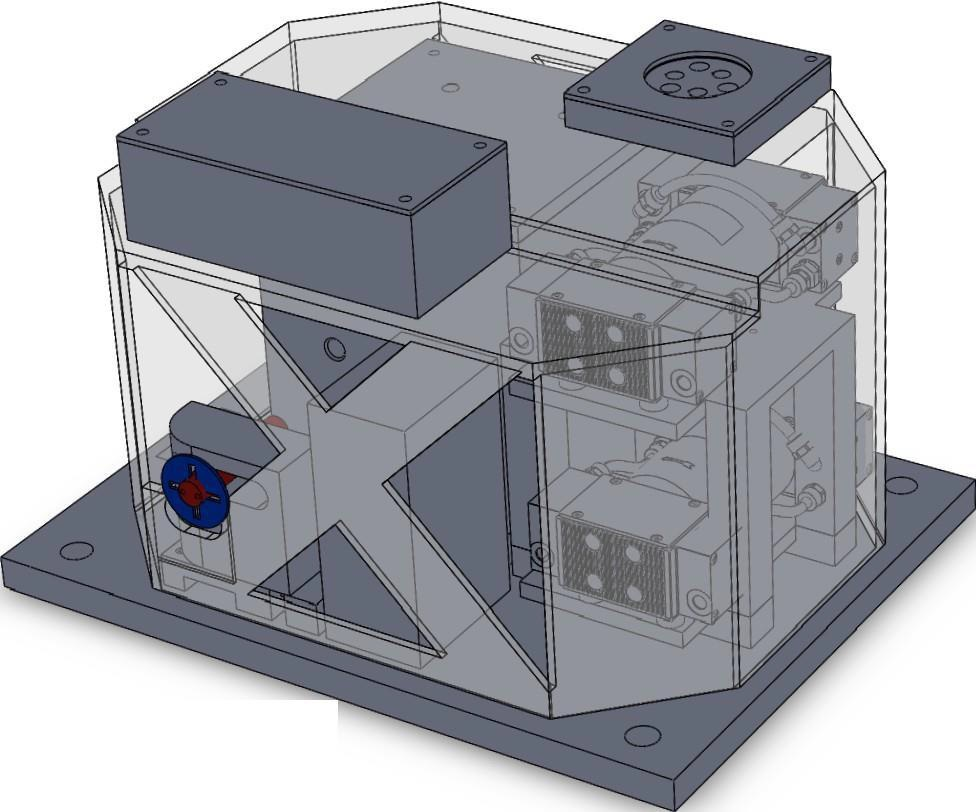
\includegraphics[width=1\textwidth]{./Figures/payload_1.jpg}
\caption{Solidworks design of the SORA payload.}
\label{fig:payload} 
\end{center}
\end{figure}
		\subsection{RESU Design}
\label{sec:RESU-Design}

For this mission, it will be necessary to build a flight computer that can manage flight operations as well as send and receive serial uplink and downlink packets.  This was the motivation for the development of a Real-Time Environmental Sensing Unit (RESU). RESU is composed of two components: a Raspberry Pi 3 (RP3) and an Arduino Mega (Arduino) which interfaced over serial USB.  The RP3 and Arduino both are hobby electronic computers, but the RP3 is geared towards recording and processing while the Arduino is more efficient at sensor integration.  The Arduino's primary purpose was to collected data from various sensors that monitored environmental conditions. It also handled telemetry, periodically downlinking packets and accepting uplink commands received from the ground. The RP3 recorded data from the Arduino's serial port and saved data frames every six seconds from the MiniPIX.  Table~\ref{tab:Sensors} lists the various sensors utilized during the flight.

\begin{table}[h!]
\centering
\caption{Table of sensors that compose RESU}
\label{tab:Sensors}
\bigskip
\begin{tabular}{|c|c|c|c|}
\hline
\multicolumn{1}{|c|}{\bfseries Sensor} & {\bfseries Quantity} & {\bfseries Platform} & {\bfseries Purpose} \\
\hline
    Temperature Sensors (TMP 36)	& 3 & Arduino  		& Record temperature measurements  \\ \hline
    Pressure        				& 1 & Arduino 		& Record pressure measurements \\ \hline
    BNO 6055       					& 1 & Arduino 		& Record IMU Data in 9 degrees of freedom \\ \hline    
    Real Time Clock 				& 2 & Arduino/RP3 	& Record temperature compensated timestamps in CT \\\hline
    Humidity        				& 1 & Arduino 		& Record atmospheric humidity levels \\ \hline
    GPS     						& 1 & Arduino 		& Determine latitude, longitude, altitude and direction \\ \hline
    MiniPIX         				& 1 & RP3     		& Cosmic ray detector \\ \hline
\end{tabular}
\end{table}

\subsubsection{Electronics Design}
Since much of the space inside of our payload was taken up by the pump and clean box from the astrobiology systems we had to design our electronics to be relatively compact.  It was decided that we would only use one RP3 to both interface with MiniPIX and store sensor data from the Arduino, rather than having one for each system as was planned originally.  Also, in order to reduce the space required for the interface between the Arduino and all of the payload's sensors, we used two layers of proto shields to more effectively utilize vertical space.  The RTC, pressure, humidity, and inertial measurement sensors were all mounted directly on the first shield while the temperature and GPS sensors were mounted on to the top most shield. 

\subsubsection{Telemetry}
RESU was designed to handle every component of the mission.  It was also in charge of all  telemetry to and from the HASP systems.  Downlinked packets provided timestamped readings from all the payload's sensors which helped us analyze the current state of our payload.  RESU also was programmed to receive four uplink commands: heaters on/off and pumps on/off.  These commands were sent at our discretion which allowed us to manage our collection systems at any given point during the flight based on environmental and component temperatures. 

		\subsection{Astrobiology System Design}
\label{sec:Astrobiology Design}
%Fre'Etta, I think we need to mention the design change to the pump and clean box, since it was a big change that affected our mission objectives


The collection assembly was initially designed as a four-compartment structure, with two collection and two control containers, two pumps, two pump heaters, and two solenoids. Due to weight and current draw  limitations, the assembly was redesigned as a two-compartment structure, with one collection and one control container,  one pump, one heater and two solenoids. The clean box and containers were machined from impact-resistant UHMWPE~\cite{cleanbox}. The control container was connected to a solenoid that remained closed until post-sanitation procedures were performed. The sample collection container was connected to a vacuum pump located outside of the clean box structure. The heater was attached to the pump to prevent a cold start. Once float altitude was reached, the solenoid connected to the sample collection container was opened and the pump was powered on; allowing air to flow to the collection container. Each container held \SIrange{30}{40}{\milli\liter} of a \SI{15}{\%} sterile glycerol solution. A 316 Stainless Steel \SI{1/4}{\inch} NPT Vent to Atmosphere Vitron Seal Valve was embedded in each of the compartments, to accommodate for the pressure changes that occurred with the variations in altitude over the course of the flight~\cite{valve}, as well as operate as the sample exhaust.  The left side of Figure~\ref{fig:pump} displays the clean box structure, showing the bottles inside and the lids with the openings for the sample and exhaust tubing, while the right side of Figure~\ref{fig:pump} shows the 3D rendering of the sampling pump. 


\begin{figure}[H] 
\begin{center}
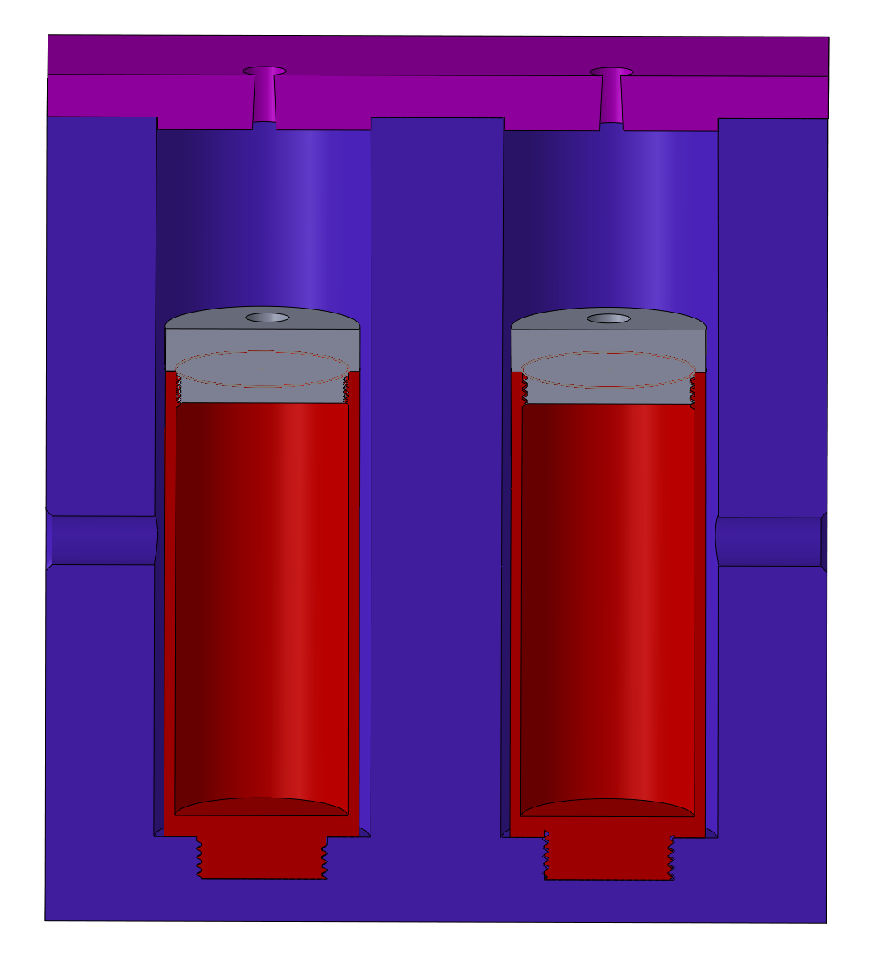
\includegraphics[scale=.4]{./Figures/CB.PDF}
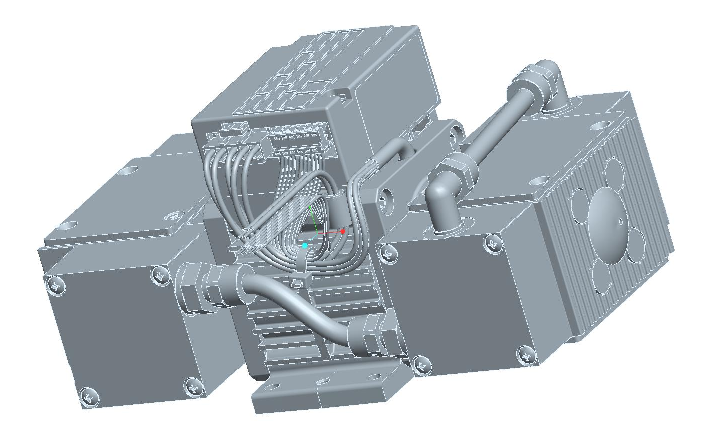
\includegraphics[scale=.8]{./Figures/Pump.pdf}
\caption{{\bf Left:} Cross-section view of the clean box with experimental and control containers. {\bf Right:} KNF N84-4 commercial gas-sampling diaphragm vacuum pump.}
\label{fig:pump}
\end{center}
\end{figure} 

		\subsection{Radiation Monitoring System}
\label{sec:Radiation Design}
\subsubsection{MiniPIX Detector}
%cite{advacam} is getting an error, leave blank and add comment
The MiniPIX detector, shown in Figure~\ref{fig:minipix} is a silicon-based hybrid pixel detector built by ADVACAM~\cite{advacam} that utilizes technology developed by the MediPIX2 collaboration at CERN~\cite{medipix}. The sensor is composed of a pixellated silicon sensor integrated with a single TimePIX readout chip (256 x 256) pixels with a pitch of \SI{55}{\micro\meter}, the layers of the detector are shown in Figure~\ref{fig:minipixlayers}. The sensor is \SI{500}{\micro\meter} thick and uses a USB 2.0 interface with a readout rate up to 30 frames per second. Each pixel can be programmed to work in one of three modes: Single particle counting, Time-over-Threshold (TOT), or Time-of-Arrival (TOA). This device offers a variety of applications including X-ray and neutron imaging as well as particle identification by characterizing each particle due to their charge, energy, and direction.

\begin{figure}[H]
  \begin{minipage}[c]{0.40\linewidth}
    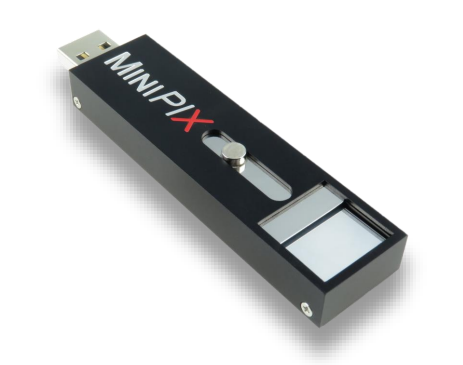
\includegraphics[width=\linewidth]{Figures/minipix_detector.png}
    \caption{Picture of a MiniPIX particle detector~\cite{advacam}.} %make sure to put figure names underneath the pictures
    \label{fig:minipix}
  \end{minipage}
  \hfill
  \begin{minipage}[c]{0.45\linewidth}
    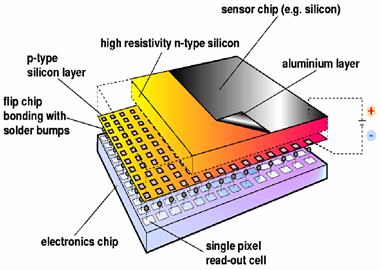
\includegraphics[width=\linewidth]{Figures/Silicon_sensor.png}
    \caption{Hybrid pixel detector silicon sensor~\cite{silicon_sensor}.} %make sure to put figure names underneath the pictures
    \label{fig:minipixlayers}
  \end{minipage}
\end{figure}

The MiniPIX registers ionized particles when the active material in the detector is transformed into a charge (the excitement of electron-hole pairs in the semiconductor). When these charges are collected, the Si bulk is then depleted by an applied bias voltage, which occurs when the electronics reads-out electron-hole pairs. If these pairs are above the threshold when collected by the pixel electronics, the count increases. The projection of the deposited charge is measured and the total energy deposited can be determined from the back-plane pulse amplitude. 

When a particle is incident on the sensor, a particle track is produced along the path length through the sensor area. The path of a single particle through the sensor is called the particle track.  Each particle track may be identified as a ``cluster'' or continuous area of neighboring pixels in a given frame. Each individual cluster can be differentiated through statistical analysis to describe the shape and energy deposition, allowing us to distinguish between different types of radiation by organizing each cluster into aspecific morphological category. 
%The feature parameters of this detector provides detailed information about total energy deposited by particles, and if only one particle is traced in the detector this tells us that slow heavy particles ionize more than fast moving ones. 

\begin{figure}[]
  \begin{minipage}[c]{0.49\linewidth}
    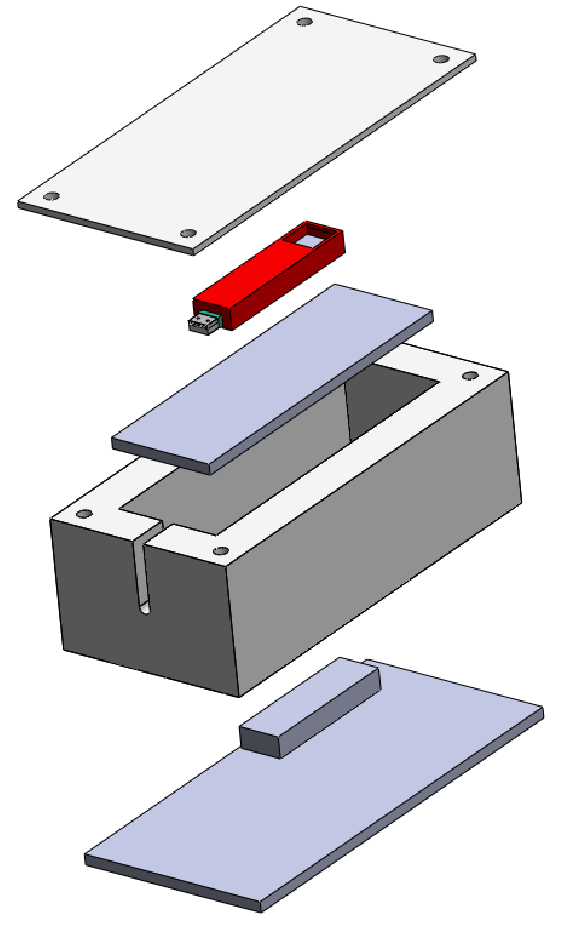
\includegraphics[scale=1, width=.5\textwidth]{Figures/Minipix_case_assembly.pdf}
    \caption{3D rendering of the MiniPIX case and heat sink assembly.} %make sure to put figure names underneath the pictures
    \label{fig:case_assem}
  \end{minipage}
  \hfill
  \begin{minipage}[c]{0.49\linewidth}
    \centering
    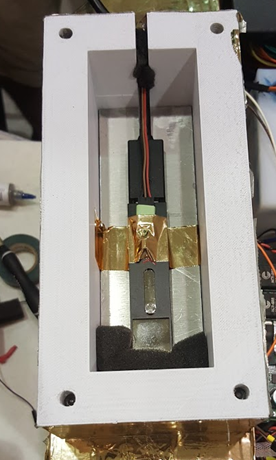
\includegraphics[scale=1, width=.5\textwidth]{Figures/minipix_mounted.png}
    \caption{Picture of the MiniPIX mounted in the case and heat sink assembly on SORA 1.0.} %make sure to put figure names underneath the pictures
    \label{fig:case_assem_pic}
  \end{minipage}
\end{figure}

The primary purpose of the MiniPIX is to detect four specific types of radiation: alpha $(\alpha)$, electron $({e^-})$, gamma $({\gamma})$, and muon $({\mu})$. By comparing the results of the flight to results obtained from simulations, an estimate regarding the percent composition of the detector hits can be made.

The MiniPIX case and heat sink assembly shown in Figure~\ref{fig:case_assem} is designed to protect the device from any moisture in the atmosphere. The case and lid will be 3D printed using ABS plastic and the heat sink will be composed of two large sheets and a small block of aluminum metal which will all be mounted to the roof of the payload. Thermal paste will be applied at every contact point between the device and each of the aluminum pieces to allow for optimal thermal conduction and radiation of heat away from the MiniPIX. A picture of the MiniPIX device inside the case and heat sink assembly used on SORA 1.0 is shown in Figure~\ref{fig:case_assem_pic}. Considering the success of that setup, we will mimic a similar configuration on SORA 2.0.

%\subsubsection{UV Photodiode Array}
%The UV photodiode array is composed of three SiC UV Photodiodes~\cite{JIC 139}. The characteristics of the photodiodes allow measurements within the spectral range between \SI{210}{\nano\meter} - \SI{390}{\nano\meter}. The maximum irradiance allowed for measurement is \SI{189}{\milli\watt\per\meter\squared}. A layer of two UV neutral density (ND) filters~\cite{Thor Labs} with optical densities (OD) 1.3 and 2.0 were positioned above each diode to reduce the transmission of UV light entering the sensor window. 3D renderings of the apparatus and filter are shown in Figures~\ref{fig:UVArray} and~\ref{fig:NDFilter}. This setup ensured that saturation of the diodes would not occur.

%\begin{figure}[!h]
  %\begin{minipage}[c]{0.49\linewidth}
    %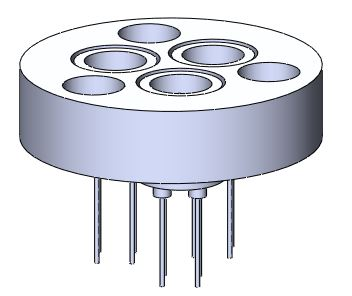
\includegraphics[scale=1, width=.5\textwidth]{Figures/uvapparatus.JPG}
    %\caption{3D rendering of the UV photodiode array.} %make sure to put figure names underneath the pictures
   % \label{fig:UVArray}
  %\end{minipage}
  %\hfill
  %\begin{minipage}[c]{0.49\linewidth}
   % 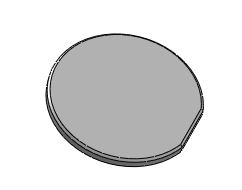
\includegraphics[scale=1, width=.5\textwidth]{Figures/uv_filter.JPG}
  %  \caption{3D rendering of an unmounted UV ND filter.} %make sure to put figure names underneath the pictures
 %\label{fig:NDFilter}
%\end{minipage}
%\end{figure}

%\subsubsection{Cosmic Radiation Methods}
%\label{sec:Radiation Methods}

\subsubsection{Calibration}   
The appropriate calibration of the MiniPIX detector will be applied at The University of Houston by Dr.~Stuart P.~George, a collaborator within the MediPIX Collaboration. The source calibration will be applied using the \SI{60}{\keV} {\ce{^241Am} decay line, \ce{Sn} Fluorescence and \ce{^55Fe} gamma rays. The TimePIX hybrid pixel detector consists of \num{65536} silicon p-n diodes, with each containing its own individual processing circuit. The response of each pixel can never be identical, thus a calibration must be performed for each individual pixel. Dr.~George will calibrate the pixel energy threshold from DAC counts to energy~\cite{stuartthesis}. The threshold will be set at \SI{4}{\keV}, just above the noise level of the detector. The set threshold energy of the TimePIX chip determines what energies of particles are allowed to be measured by the detector. Energy measurements in the detector are accounted by measuring the charge collected in each individual pixel. The sensor's bias voltage will be \SI{200}{\volt} to ensure that the sensor was completely depleted. 
  
\subsubsection{Collection Parameters}
% Put the settings for the minipix shutter time, bias voltage etc. here
%The device will be configured via the device Python API wrapper provided by ADVACAM. Acquisition parameters will be determined through testing. This time must be chosen as a balance between too many individual frames with little to no data, which would take up a lot of storage space, and individual frames that are so crowded with interactions that they are unreadable due to a large number of crossed tracks. Upon completing an acquisition, the device enters a manufacturer-set dormant state for approximately two seconds, which will be utilized as cool-down period and to record the internal temperature of the device into a .csv file.

\subsubsection{Data Format}
The data format for each frame of data is a plain text array with each value corresponding to the value at the corresponding pixel index in the detector. Upon the capture of a new frame the plain text array will be appended to the acquisition file stored on the SD card of the RP\num{3} on our payload. In a separate file various metadata will be stored for each frame including the detector threshold, acquisition time, acquisition mode etc. The plaintext array format means that each frame of data utilized approximately \SI{132}{\kilo\byte} of memory. In SORA \num{1.0}, a frame was saved roughly every six seconds, over the course of the roughly fourteen hour flight we had a total acquisition size of approximately \SI{1.1}{\giga\byte}. While this was a rather small total collection size, we could have further reduced our memory footprint by only storing pixel indices with non-zero time over threshold values i.e.\ storing data in a sparse matrix format. This is a route we will look into for SORA \num{2.0}.

%The Arduino from RESU was used to supply a constant \SI{5.0}{\volt} signal to each detector. When a UV photon is incident on the sensor, a photocurrent is induced in the circuit and a voltage pulse is returned to the Arduino and stored on the RP3. The sensor output current can be calculated from the measured voltage and the spectral irradiance can be calculated based on the characteristics of the detector. SORA used this apparatus to quantify the spectral irradiance of solar UV light in the stratosphere.

	%Subsystems and Functions
		%%\newpage
\section{Subsystems and Functions}
\label{sec:Methods}

%\begin{figure}[!htb]
%\begin{center}
%
\includegraphics[width=0.5\textwidth]{./Figures/Test.jpg}
%\caption{This is a test figure.}
%\label{fig:Test} 
%\end{center}
%\end{figure}
		%%\clearpage
\subsection{Electronics System Design}
\label{sec:RESU}

\subsubsection{Overview}

The RESUs primary purpose during the flight will be to monitor environmental conditions and control the astrobiology systems. It will monitor temperature of the various subsystems and the humidity and pressure of the environment throughout the flight. All recorded data will continuously be written to an SD card mounted on a shield on top of the Arduino. It will also accept discrete commands from the HASP systems to turn the astrobiology collection system on and off.

\subsubsection{The Sensors}

Our payload will utilize eight thermistors to measure temperature at various points in our payload. The decision to use thermistors was based primarily on the performance of the analog temperature sensors during our 2017 flight, during which several of those sensors failed. Thermistors are able to accurately measure temperature in the range \SIrange{-55}{125} and should therefore be adequate for the conditions in the stratosphere. Pressure will be recorded from two identical digital pressure sensors in order to ensure accuracy and should be able to record accurately in the range \SIrange{0}{14000}{\milli\bara}. Finally, humidity will be measured from a basic analog humidity sensor. All sensor data will be UTC timestamped via the onboard Real Time Clock and recorded to the SD card.

 %UVC radiation was measured by three identical sensors.  They supported light ranging from \SIrange{210}{380}{\watt\per\square\meter} and were located outside the roof of the payload.  These sensors were analog so their readings were voltages induced by incident rays on the surface of each sensor. To stabilize the voltage readings from each sensor, a \SI{3300}{\micro\farad} capacitor was placed across the ground and analog out pins of the sensor.  Data was collected every \SIrange{3}{4}{\second}.


\subsubsection{Powering It All Up}

In order to stay within the power constraints, a robust power supply will need to  handle all the components of the payload.  The power supply we will be using is the PPM-DC-ATX-P by WinSystems INC.  It offers the desired number of \SI{+5}{\volt} and \SI{+12}{\volt} outputs needed to power the payload's electronics.  This power supply could effectively take \SI{+30}{\volt} and step it down to two \SI{+12}{\volt} and two \SI{+5 }{\volt} outputs.  One of the \SI{+12}{\volt} outputs goes to the Arduino since it can step down to the appropriate voltages internally while the other goes to a PWM motor for the solenoid.  One of the \SI{+5 }{\volt} outputs powers two analog sensors that will be sent to HASP through the EDAC connection (more on that in the next sections).  The remaining \SI{+5 }{\volt} output is converted to a USB power cable for the RP3.  The power supply also has four ground outputs that will be used by each respective component. 


%Listing~\ref{Downlinks} is a sample downlink data packet received during our previous flight.

%\lstset{basicstyle=\small, numbers=left, xleftmargin=2em, frame=tb, label = Downlinks, framexleftmargin=1.5em}
%\begin{lstlisting}[caption = Sample of downlinked data packets ID: 15667 - 15670 from SORA 2017~\cite{SORA}.]
%...
%begin_packet
%15667,-21.05,-0.33,35.62,-1.00,0.12,0.25,-0.71,0.63,9.30,-30.25,-26.69,-60.88
%3.14,2.86,0.00,0.00,0.60,9:29:39 9/4/17
%end_packet
%begin_packet
%15668,-20.95,-0.54,35.62,0.75,0.06,-0.69,0.25,-2.00,9.67,-28.37,-28.06,-60.06
%3.80,3.33,0.00,0.00,0.60,9:29:42 9/4/17
%end_packet
%begin_packet
%15669,-21.15,-0.54,35.62,0.81,-0.06,-0.56,1.22,-2.13,9.86,-29.56,-27.75,-57.88
%1.86,2.86,0.01,0.02,0.61,9:29:45 9/4/17
%end_packet
%begin_packet
%15670,-21.15,-0.54,35.62,-1.00,0.00,0.12,-0.55,0.73,9.37,-27.37,-30.00,-58.75
%1.86,3.96,0.00,0.00,0.61,9:29:48 9/4/17
%end_packet
%...
%\end{lstlisting}
%\medskip
%
%Each packet of data will be delimited by keywords \verb|begin_packet| and \verb|end_packet| so that parsing each file be easier.  During our previous flight, these data packets were crucial status updates to the state of our payload.  We will once again use them for the same purpose to keep a close eye on our payload.
%
%Data packets will contain information about the readings from each sensor.  The first integer represents the ID of the packet.  Following the packet ID are the three temperature readings, gyroscope $x, y, z$ values, accelerometer $x, y, z$ values, magnetometer $x, y, z$ values, pressure readings, humidity readings, UV \#1, \#2, \#3 voltage readings, and finally the timestamp in $HH$:$MM$:$SS$ $MM$/$DD$/$YY$ at which the packet was written.  
%
%In addition to downlinking sensor data, we also want to downlink serial uplink commands as shown in listing \ref{Uplinks}.  
%
%\lstset{basicstyle=\small, numbers=left, frame=tb, linewidth=11.5cm, xleftmargin=.4\textwidth, label = Uplinks}
%\begin{lstlisting}[caption = Sample of received uplink commands in downlinked packets in SORA 2017~\cite{SORA}]
%...
%1
%2
%71
%FFFFFFFF
%3
%D
%A
%Received Command: 71
%...
%\end{lstlisting}
%\medskip
%
%Each line within a received uplink command represents the string of bytes that will be read by our payload.  The last line of the listing shows what command will be parsed and processed by RESU.  Table \ref{tab:All-Commands} shows all the possible commands that we are expecting to process. 

			%Data Interface
			%HASP and Paylad Communication
			%Uplink Data Format
			%Downlink Data Format
		%\subsection{Astrobiology Methods}
\label{sec:Astrobiology Methods}

\subsubsection{Vacuum Chamber Testing}
\label{subsec:Astro Vacuum}


The pumps, along with the temperature, humidity and pressure sensors and tubing will undergo extensive thermal vacuum testing in the range of \SIrange{-3}{25}{\celsius}, with a pressure range of \SIrange{0}{10}{\milli\bar}. The vacuum chamber tests will run for approximately \SIrange{8}{15}{\hour}, to replicate conditions from the previous flights. In the past~\cite{SORA}, the pumps were subjected to a temperature range of \SIrange{-30}{50}{\celsius} during integration and ran again for \SI{8}{\hour} afterwards and prior to flight. The pumps have proven to function in extremem environments without an issues. 


\subsubsection{Pre-Flight Preparation}


The clean box, collection containers and tubing will be autoclaved. All tools used in the assembly of the clean box will either be autoclaved or soaked in a \SI{70}{\percent} ethanol solution inside of a clean room. Each person who enters the clean room will be garbed in a lab coat, goggles, hair net and latex gloves after thoroughly washing their hands in a \SI{70}{\percent} ethanol solution. 

%We need to reword this to fit what Dr. Pattison wants us to do now that we have her onboard

%The \SI{15}{\percent} glycerol solution will poured into each container, the lid was sealed with silicone gasket maker and the tubing was inserted and gasket sealed into the container lids. Each lid had two holes, one that led to the inside of the clean box to allow for pressure to be released from inside the container and outgassed through the valve embedded in the box, while the other hole passed through the clean box lid to allow the tubing to connect to the pump or solenoid only in the case of the control tubing. The lid to the clean box was sealed with silicone gasket maker, the box was then mounted onto the payload and the tube from the control container was clamped to the dedicated control solenoid, while the sample collecting tube was passed through the other solenoid and connected to the pump. A final piece of tubing was connected from the intake valve on the pump to the outside of the payload, after a \SI{70}{\percent} ethanol solution was run through the pump several times. The end of the tube was bent, and zip tied. The payload was closed and remained in the clean room until it was ready for transport to Fort Sumner.  At the launch site, the zip tie was cut and the exposed inner and outer tubing was swabbed with an alcohol pad approximately \SI{4.5}{\hour} prior to launch. 



\subsubsection{Post Flight Procedures}

%Reword this section too to match what we plan to do after we recover it.  Include first that we will put the cleanbox in an iced cooler.

%The payload was successfully retrieved on September~6,~2017. The intact clean box was removed and placed inside of a cooler with ice, transported to The University of Houston and placed in cold storage at \SI{4}{\celsius}. All equipment used in the filtration process was either autoclaved or taken from previously unopened sanitized packaging. The autoclaved, pre-sanitized items and the clean box were washed in a \SI{70}{\percent} ethanol solution before they were placed inside a SterilGARD e3 Class II Biological Safety Cabinet. The Cabinet has a laminar flow air barrier and UV lights built into the ceiling for decontaminating the workspace prior to use. Both the control and sample collection solutions were vacuum filtered through a Fluropore membrane filter (\SI{13}{\milli\meter}; \num{0.22} micron) to collect specimens on the filter surface.  The filters were packaged for shipment to RTL Genomics~\cite{RTL} for 16S ribosomal RNA sequencing. All post flight sanitation and sample and control filtration procedures took place under the supervision of Professor Donna Pattison from the Department of Biology and Biochemistry at The University of Houston.


%\subsubsection{Ribosomal RNA Sequencing and Data Analysis}
%
%
%
%We sent our filtered control and experimental samples to RTL Genomics in Lubbock, Texas for ribosomal RNA sequencing and data analysis. We selected the 926wF  (``AAACTYAAAKGAATTGRCGG'') and 1392R (``ACGGGCGGTGTGTRC***'') primers for the sequencing procedure. These primers are designed to amplify 16S RNA from bacterial, archaeal and eukaryotic ``universal'' samples. The samples were amplified using a two step PCR procedure~\cite{lemon}. Samples were sequenced on an Illumina MiSeq~\cite{illumina} 2x300 flow cell at 10~pM and sequenced at RTL Genomics using standard sequencing procedures~\cite{Microbial rRNA sequencing}.


%		\subsection{Cosmic Radiation Methods}
\label{sec:Minipix Testing}
	
	\subsubsection{Calibration}   
	The appropriate calibration of the MiniPIX detector was applied at The University of Houston by Dr.~Stuart P.~George, a collaborator within the Medipix Collaboration. The source calibration was applied using the \SI{60}{\keV} {\ce{^241Am} decay line, \ce{Sn} Fluorescence and \ce{^55Fe} gamma rays. The Timepix hybrid pixel detector consists of \num{65536} silicon p-n diodes, with each containing its own individual processing circuit. The response of each pixel can never be identical, thus a calibration must be performed for each individual pixel. This is a fairly complicated procedure and was our first setback. Originally, the device should have shipped with an energy calibration from the manufacturer, but we had issues with the provided energy calibration.

	The data was recorded using the Pixet Pro software provided by ADVACAM~\cite{advacam}. Dr.~George calibrated the pixel energy threshold from DAC counts to energy~\cite{stuartthesis}. The threshold was set at \SI{4}{\keV}, just above the noise level of the detector. The set threshold energy of the Timepix chip determines what energies of particles are allowed to be measured by the detector. Energy measurements in the detector are accounted by measuring the charge collected in each individual pixel. 

	
	\subsubsection{Thermal Vacuum Testing}
	 In near vacuum environments, electrical devices under continuous operation tend to build up heat as there is practically no thermal convection. The MiniPIX under normal atmospheric pressure has very little variance in temperature, but during vacuum testing performed at The University of Houston and during integration at the Columbia Scientific Balloon Facility the device proved to heat up to temperatures above the maximum recommended operating temperature of \SI{70}{\celsius}. Although the device is designed to operate between \SIrange{0}{70}{\celsius}, our testing proved that it could continue to function well beyond either side of these limits~\cite{mpdatasheet}. Regardless, after the first day of thermal vacuum testing during integration in Palestine, TX, it was decided to fit an aluminum heat sink to the MiniPIX to better regulate its temperature. During the second day of testing the heat sink we fitted proved to be highly effective and the temperature of the MiniPIX did not dip below  \SI{5}{\celsius} and did not exceed  \SI{37}{\celsius}.

	\subsubsection{Collection Parameters}
        % Put the settings for the minipix shutter time, bias voltage etc. here
  	The device was configured via the device Python API wrapper provided by ADVACAM. The particle energy threshold was set to \MPThreshold, which prohibited the sensor from registering energy values that were less than the set value. Acquisition parameters were set to have a shutter time of four seconds per frame, meaning the device records four seconds' worth of data for each frame. This time was chosen as a balance between too many individual frames with little to no data, which would take up a lot of storage space, and individual frames that are so crowded with interactions that they are unreadable due to a large number of crossed tracks. Upon completing an acquisition, the device would enter a manufacturer-set dormant state for approximately two seconds, which was utilized as cool-down period to record the internal temperature of the device into a .csv file. The sensor's bias voltage was chosen to be \SI{200}{\volt} to ensure that the sensor was completely depleted. 

\subsubsection{Data Format}
The data format for each frame of data is a plain text array with each value corresponding to the time over threshold value at the corresponding pixel index in the detector. Upon the capture of a new frame the plain text array was appended to the acquisition file stored on the SD card of the RP3 on our payload. In a separate file various metadata was stored for each frame including the detector threshold, acquisition time, acquisition mode etc. The plaintext array format means that each frame of data utilized approximately 132 KB of memory. With a frame being saved roughly every six seconds, over the course of the roughly fourteen hour flight we would expect to see a total acquisition size of approximately 1.1 GB. While this is a rather small total collection size, we could have further reduced our memory footprint by only storing pixel indices with non-zero time over threshold values i.e.\ storing data in a sparse matrix format. 

\subsubsection{Clustering Algorithm}  	
\begin{figure}
 	\begin{center}
 	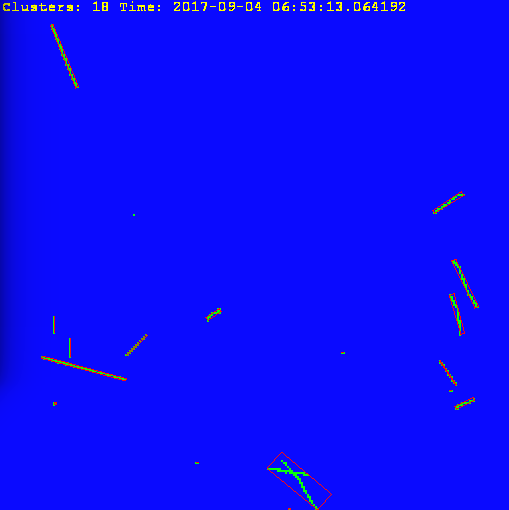
\includegraphics[width=0.5\textwidth]{./Figures/crossedtracks.png}
 	\caption{Frame with two detector hits with crossing paths (bottom-center and shown inside red box).}
 	\label{fig:crossedtracks}
 	\end{center}
\end{figure}

  	Given our raw data frames after flight we needed to perform a clustering algorithm to break up each frame of data into a series of relevant parameters for each individual particle hit. It was decided that given its ease of development we would implement this algorithm in Python utilizing the Numpy scientific computing library~\cite{numpy}. While lacking the speed of C/C++, Python allowed us to quickly develop and debug the algorithm so that we could have more time to analyze the results. However, what we gained in implementation speed we lost in execution time and interactivity. Python proved to be quite slow compared to a compiled language and was rather clumsy in terms of providing interactive plots. It also took many hours each time we wanted to reanalyze our flight data. We could have avoided much of this by either writing the more processing intensive algorithms in C and creating hooks into our Python code or by simply writing the entire algorithm in C or C++.

The clustering algorithm we used was a fairly straight forward flood fill implementation. We considered a cluster to be a contiguous region of pixels that registered a non-zero value. Thus, we iterated over each pixel in a frame and performed flood fill on any pixel that had not already been checked and had a non-zero value. The indices and value for each member of a contiguous region was then stored for later processing. This approach worked very well for the most part, except for when tracks from two different hits crossed, which caused two separate detector hits to be counted as one. This issue, shown in Figure~\ref{fig:crossedtracks}, occurred periodically throughout the flight but especially during ascent when cosmic ray intensity was at its peak. While this is a hard limitation of hybrid pixel detectors, a shorter frame exposure time could have prevented this issue during the high rate periods.



\subsubsection{Cluster Sorting Algorithm and Morphological Analysis}

Based on guidance from Dr.~George, who wrote his doctoral thesis on a hybrid pixel detector similar to the MiniPIX~\cite{stuartalgo}, we implemented a cluster sorting algorithm that sorts hits on our detector based on the pixel count, pixel density and the ratio between the length and width of the clusters bounding box. The algorithm we implemented, is nearly identical to the one developed by Dr.~George and outlined in Figure~\ref{fig:sortingalgo}. The only major difference is that, because of the thickness of the silicon chip of our MiniPIX detector, we had to increase the number of inner pixels from \num{4} to \num{8} to increase our heavy track discrimination. This is due to the fact that the original algorithm was tuned for a \SI{300}{\micro\meter} thick detector while our MiniPIX is \SI{500}{\micro\meter} thick, which resulted in thicker tracks. In general the morphological characteristics of a track left on the sensor can give us a good idea of the possible type of particle that hit the detector. For example a straight t rack on the detector is possibly explained as being deposited by a muon, fast proton or pion.

	\begin{figure}[h!]
 	\begin{center}
 	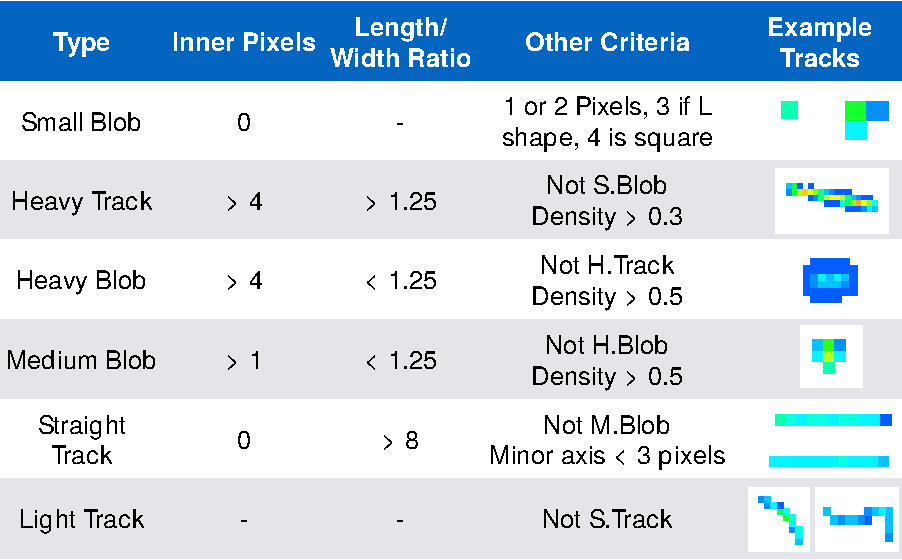
\includegraphics[width=0.75\textwidth]{./Figures/stuartgraphic.pdf}
 	\caption{Morphological characteristics used by the sorting algorithm that is based on clusters~\cite{stuartalgo}.}
 	\label{fig:sortingalgo}
 	\end{center}
 	\end{figure}
\newpage

\subsection{Solar Radiation Methods}
\label{UV Photodetector Testing}

	\subsubsection{Responsitivity and Limitations}

	The three photodiodes used for this experiment were the JIC 139 UV photodiodes with integrated amplifiers. We used the pin configuration provided by the datasheet to create an electronic circuit to integrate the photodiodes. To filter out noise, we included a \SI{3300}{\micro\farad} capacitor for each photodiode. With this configuration, we were allowed to apply a UV light source to record the measured Voltage output $V_{\text{Out}}$ with the RESU. The photocurrent $I_{\text{PD}}$ generated from incident light on the detector can be calculated by


	\begin{equation}
	I_{\text{PD}} = \frac{V_{\text{Out}}}{R_{f}}
	\label{eq:photocurrent}
	\end{equation}


	where $R_{f}$ is the internal feedback resistor. Then, with the calibrated specifications provided, we were allowed to determine the irradiance of UV light $E_{e}$ by
	
	\begin{equation}
	E_{e} = \frac{I_{PD}}{(A \cdot R)}
	\end{equation}
	

	where ${A}$ is the size of the active area and ${R}$ is the spectral responsitivity. The specifications and internal components that make up the photodiode determine the peak irradiance or limit of saturation where the voltage supplied (\SI{5}{\volt}) is equal to the voltage out. We used this value in Equation~(\ref{eq:photocurrent}) to calculate a maximum irradiance of \SI{189}{\milli\watt\per\square\meter} as shown in Table~\ref{tab: UV-Specs}.


	\begin{table}[h]
	\centering
	\caption{Specifications and peak irradiance of the UV photodiodes.}
	\label{tab: UV-Specs}
	\bigskip
	\begin{tabular}{|c|c|c|c|c|}
	\hline
	\multicolumn{1}{|c|}{\bfseries Parameters} & \multicolumn{1}{|c|}{\bfseries JIC 137} &    \multicolumn{1}{|c|}{\bfseries JIC 138} & \multicolumn{1}{|c|}{\bfseries JIC 139} & \multicolumn{1}{|c|}{\bfseries Unit}\\
	\hline
	    Active Area $(A)$         		& $0.22$  		& $0.22$ 	& $0.22$ 	& \si{\square\milli\meter} 			\\ \hline
	    Max Responsivity $(R)$    	& $0.12$  		& $0.12$ 	& $0.12$ 	& \si{\ampere\per\watt}  		\\ \hline
	    Feedback Resistor $(R_f)$ 	& $10$    		& $100$  	& $1000$ 	& \si{\mega\ohm} 				\\ \hline    
	    Output Voltage $(V_{OUT})$ & $5$     		& $5$    	& $5$    	& \si{\volt}      					\\ \hline
	    Photocurrent $(I_{PD})$     	& $500$   		& $50$   	& $5$	& \si{\nano\ampere}        			\\ \hline
	    Peak Irradiance $(E_e)$   	& $18939$ 	& $1849$ 	& $189$  	& \si{\milli\watt\per\square\meter}     	\\ \hline 
	\end{tabular}
	\medskip
	\end{table}

	%The standard solar spectrum known as $AM0$ was integrated over the Sun's UV spectrum ${S}{(\si{lambda})}$ from $210\si{\nano\meter}$ $380\si{\nano\meter}$.

	The irradiance of UV light increases by about \SI{6}{\percent} per kilometer of altitude and may vary depending on the amount of ozone~\cite{uv_irradiance} in the local region. The UV ND filters were added to the aperture to ensure the diodes would be able measure the high UV irradiance in the stratosphere. The total optical density ${(OD_{\text{Tot}})}$ can be determined by the sum of the filters ${OD_{1}}$ and ${OD_{2}}$. The optical density for one filter can be determined by

	\begin{equation}
	OD =  {log}_{10} (\frac{1}{T})
	\end{equation}
	
	where $T$ is the percent transmission of the filter in the UV region provided by Thor Labs.

		\section{HASP Interface}
\label{sec:Hasp-Interface}

\subsection{Interfacing With HASP: Serial Uplink and Downlink}
During the duration of our flight the serial uplink commands will be used to configure the collection parameters of the MiniPIX radiation detector. When a command is received from the mission control team, it will be transmitted straight through the DB9 connection into the RPI3 through an RS232 to ttl converter. Then the monitoring script on the RPI3 will verify its content and perform the appropriate action defined in Table~\ref{tab:All-Commands}. The baud rate for serial communication will be set to 4800 bits per second ($bits/sec$). 


\begin{table}[!ht]
\centering
\caption{Table of All Uplink Command} 
\label{tab:All-Commands}
\bigskip
\begin{tabular}{|c|c|c|c|}
\hline
\multicolumn{1}{|c|}{\bfseries Command} & \multicolumn{1}{c|}{\bfseries HEX Uplink Command} & \multicolumn{1}{c|}{\bfseries HEX Uplink Argument}\\
\hline
    Begin Acquisitions 		& 0x01	 & N/A			    	    \\ \hline 
    Stop Acquisitions 		& 0x02	 & N/A			            \\ \hline
    Set Shutter Time		& 0x03   & Shutter Time in seconds (1-255)  \\ \hline %two pumps now
    Change Acquisition Mode    	& 0x04 	 & HEX Mode Identifier 	            \\ \hline
    Device Reset		& 0x05 	 & N/A				    \\ \hline
    
\end{tabular}
\medskip
\end{table}

\begin{table}[!ht]
\centering
\caption{Table of Acquisition Modes} 
\label{tab:Acq-Commands}
\bigskip
\begin{tabular}{|c|c|c|}
\hline
\multicolumn{1}{|c|}{\bfseries Acquisition Mode} & \multicolumn{1}{c|}{\bfseries Hex Mode Identifier} & \multicolumn{1}{c|}{\bfseries Description}\\
\hline
    Automatic Shutter Time	& 0x01   & Shutter time determined automatically based on particle flux   \\ \hline %two pumps now
    Fixed Shutter Time    	& 0x02 	 & Shutter time fixed to set shutter time 	     		  \\ \hline
    Counting Mode    		& 0x03 	 & Configure MiniPIX to measure counts on the detector only 	  \\ \hline
    ToT Mode			& 0x04	 & Configure MiniPIX to measure time over threshold values	  \\ \hline
    ToA Mode			& 0x05 	 & Configure MiniPIX to measure time of arrival 	     	  \\ \hline
\end{tabular}
\medskip
\end{table}


\subsection{Interfacing with HASP: EDAC and DB9 Connections}

Our wiring will not change much from the last mission~\cite{SORA}.  From the EDAC pins, we will join two of the \SI{30}{\volt} leads together in parallel to supply power to the central power supply.  Likewise, two of the ground leads will be used to ground the supply.  A pair of \SI{30}{\volt} and ground leads will also be used as input to the relay circuit in order to supply power to the pumps which require at least \SI{24}{\volt} to operate.  The last pair of \SI{30}{\volt} and ground leads will be used as input to the punch and hold circuit mentioned in the previous section to power the solenoids which require at least \SI{20}{\volt} to operate.  Two temperature sensors will be connected by both analog leads from the EDAC connection.  The corresponding ground pins will be used to ground them.  These two sensors will be placed on each of the pumps.

We will use discrete commands in this mission.  Two of the commands will be used to turn the astrobioly system on and off.  This is only in case of emergency if we notice that the system is not responding to our serial commands.  The other two discrete channels will be used to turn on and off the power of RESU in case that we notice an issue.

\begin{table}[!ht]
\centering
\caption{Table of all discrete commands to be used during flight} 
\label{tab:Dis-Commands}
\bigskip
\begin{tabular}{|c|c|c|c|}
\hline
\multicolumn{1}{|c|}{\bfseries Command} & \multicolumn{1}{c|}{\bfseries Purpose} &  \multicolumn{1}{c|}{\bfseries EDAC Pin} & \multicolumn{1}{c|}{\bfseries Description} \\
\hline
    Discrete 1     	& Astro. System ON 	& f	 & Initiates the pumps and collection systems   \\ \hline 
    Discrete 2    	& Astro. System OFF 	& n	 &  Shuts down the pumps and causes collection systems to retract  \\ \hline
    Discrete 3  	& RESU On 	& h	 & Powers up RESU   \\ \hline 
    Discrete 4 		& RESU OFF 	& p	 & Shuts down RESU   \\ \hline
\end{tabular}
\medskip
\end{table}


	%Thermal Control Plan
		\section{Thermal Control Plan}
\label{sec:TCP}
Based on our previous mission~\cite{SORA}, we opted to have a similar thermal control plan but with a few changes.  To simplify the payload construction and control, we opted for an semi-autonomous temperature monitoring and control system.  

The Arduino will monitor the pumps and other devices for overheating.  If the Arduino detects that a components, such as the pumps, then it will shut down the whole astrobiology system for a certain amount of time.

In the case of our payload experiencing colder temperatures, all of our devices will be able to operate beyond expected temperatures on the flight. Based on our previous mission~\cite{SORA}, we found that heaters were not needed, just insulation.

The temperature will be checked and recorded periodically for all devices, but it will not be downlinked.

In order to manage the temperature of the  MiniPIX will be fitted with the same heatsink configuration as our 2017 flight. The internal temperature of the device will be recorded and downlinked to the flight control team at regular intervals. If the device is beginning to experience temperatures beyond what we would consider safe (above \SI{70}{\celsius}) we can either reset the RPI3 controlling the MiniPIX or fully shutdown the entire radiation subsystem.

%\begin{figure}[!htb]
%\begin{center}
%
\includegraphics[width=0.5\textwidth]{./Figures/Test.jpg}
%\caption{This is a test figure.
%}
%\label{fig:Test} 
%\end{center}
%\end{figure}

	%Sensors
	%Power Budget & Weight Budget
		\section{Power and Weight Budget}
\label{sec:PW_Budget}
We will copy the thing from the provisional application and update it with new values....



%Testing and Simulation
\section{Procedures}
\label{sec:Procedures}

\subsection{Decontamination and Blah}
\label{subsec:Decontamination}

\subsubsection{Objectives:}
Sanitization procedures are critical. They need to be checked and verified to ensure that our samples will not become contaminated. If the samples were to become contaminated it would make any possible bacterial collection data inconsequential.

\subsubsection{Sterilization Preflight:}
The payload will be built within the confines of a class 100 clean hood that is located inside of a class 10,000 clean room. Any tools that are used to construct the sampling box will be heat sterilized at \SI{120}{\celsius} for \SI{20}{\minute}. This will be followed by exposing each side of the container to germicidal UV-C (\SI{254}{\nano\meter}) light for \SI{20}{\minute} and then soaked overnight in 91\% isopropyl alcohol to denature proteins in any possible sources of contaminating bacteria. This sterilization method destroys close to 100\% of all organisms and their endospores. To sterilize parts that would otherwise be damaged by the autoclave method they will be cleaned by hand with 91\% isopropyl alcohol to kill microorganisms by denaturing proteins and dissolving the lipid membrane. Following this, the materials will be rinsed with a 95\% ethanol (v/v) solution as an extra precautionary step to ensure complete decontamination. After all parts have dried, the sampling container will be constructed and placed in a gas-porous sterilization pouch and exposed to ethylene oxide (EO) at a concentration of 0.45-0.65 \SIrange{0.45}{0.65}{\milli\gram\per\meter\cubed} at \SI{55}{\celsius} and 30-50 \% RH for \SI{4}{\hour} to annihilate any spores and to provide another form of anti-bacterial treatment. The SMITH payload for HASP 2011 was processed in a similar fashion. Two identical chambers will be created to have a sampling container and a control container that will remain closed during the flight. This will provide a means to determine if contamination occurs. While the test sampling containers are under construction, the sterilization procedures are to be followed while under a sterilized hood, where samples will be collected to verify their contamination free status. Once the final HASP integration is ready for sampling and control containers are produced, both chambers will be sterilized and sealed. After the containers are integrated into the rest of the payload, the entire device will be placed in an autoclave bag for transportation.

\subsubsection{Sterilization Post flight:}
Before payload descent, a halt sampling command will be issued to the payload via uplink. The
halt sampling command will seal the sampling container by shutting down the pump system and closing all solenoid valves. Each team member involved in the recovery process should where new latex gloves; cleaned with 91 \% isopropyl alcohol. The payload will remain sealed until decontamination procedures are complete and the sampling container is ready for processing. The payload will be disassembled under class 100 conditions and all tools used during this procedure will be either heat or 91 \% isopropyl alcohol sterilized. Once in the clean room, the same procedures that were performed preflight will be performed post flight. The sampling box will then be packaged in a heat sterilized plastic outer container and transported to a biological facility that will then determine the quantity of cells present.

%\subsubsection{In Flight Failure:}
%If for some reason the sampling system fails, commands can be uplinked to the control system that
%allow for subsystem resets. If the temperature falls below component operating conditions, the heater associated to that particular subsystem will automatically turn on until operating conditions are restored and the system is operational. Although unlikely, if downlinked data shows extreme overheating or any sort of abnormality that could result in damage to HASP or other payloads, we will shut down all systems through the discrete command provided by HASP.

\subsection{Testing}

\subsubsection{Vacuum Chamber}
There will be an initial testing phase that will include each component that will draw or supply power/current. During this phase, each component will receive power and transmit data to ascertain proper functionality. Communication will be tested by sending commands to the system and receiving status updates in return. In addition, to testing proper functioning of the pumps and solenoid valves, the clean box will be tested to ensure sanitation procedures are successful and verify that the materials inside the bottles within the clean box remain unfrozen. This initial phase is to be followed by an integration of components into their respective subsystems. Each subsystem will be tested to ensure functionality within itself and confirm actual power consumption and current drawn at various voltages. The subsystems will be thermally vacuum tested to determine thermal stability and general functionality at each phase of the flight (ascension, float, descent) for a total of 24 hours. Finally, a complete integration will complete the payload. The complete integration will be tested in the same manner as the subsystems to establish a fully functioning payload. Once this final phase is complete, the payload will be sealed after it has undergone sanitation procedures.

\subsection{Integration Procedures}
\subsubsection{UH Integration}
For Astrobiology, we will try to determine the airflow through the system under normal ground level conditions and float conditions with as much precision as possible.  We will run two pumps and we will monitor the power consumption of the system as well. The pumps, along with the temperature, humidity and pressure sensors and tubing will undergo extensive thermal vacuum testing in the range of \SIrange{-3}{25}{\celsius}, with a pressure range of \SIrange{0}{10}{\milli\bar}. The vacuum chamber tests will run for approximately \SIrange{8}{15}{\hour}, to replicate conditions from the previous flights. In the past~\cite{SORA}, the pumps were subjected to a temperature range of \SIrange{-30}{50}{\celsius} during integration and ran again for \SI{8}{\hour} afterwards and prior to flight. The pumps have proven to function in extremem environments without an issues. 

There will be several clean boxes used during the testing procedures to ensure stability of the materials and agarose solution under flight conditions. The multiple boxes will also allow for contamination and leak testing. Once the aforementioned actuator/pump/solenoid combination has been assembled, the sealed and sanitized clean box will be connected via the tubing from the pumps. This new assembly will be vacuum chamber tested under the same pressure and temperature conditions that are to be expected throughout the flight. 

RESU will once again undergo rigorous testing in order to ensure proper operation. Once all components are collecting data we will run a test in the vacuum chamber under float conditions. If any of the sensors fail, we will gradually add components and vacuum test the system at each stage until we identify the source of the problem.

When the actuator/pumps/solenoid/clean box assembly and the environmental package assembly have undergone separate and complete flight simulations in the vacuum chamber, the two will be combined to form a more complete assembly. This new assembly will be vacuum chamber tested. 

In near vacuum environments, electrical devices under continuous operation tend to build up heat as there is practically no thermal convection. Based off of the results from the last mission, we have decided the aluminum heat sink is the best option~\cite{SORA}. Once the MiniPIX has been tested separately it will be added to the assembly to make a final assembly that will be vacuum tested. The MiniPIX will be integrated with the Raspberry Pi via USB. Using the Pixet software, we will test known sources to measure the energy levels and particle flux to ensure that the MiniPIX has been properly calibrated.
    
%Our detailed preliminary testing plan is described in \textbf{appendix B (make sure this stays consistent)}.  

\subsubsection{HASP Integration}
The integration team, which consists of all team members to date, will arrive at the integration site approximately \numrange{1}{2} days before the scheduled testd. The first step of the integration will be to attach the payload to the HASP plate. Following attachment, it will be verified that the payload receives power from the HASP EDAC connector and is successfully sending and receiving operation commands from the ground. Our results for bacteria collection rely heavily on a very little to no contamination risk setting pre and post flight, therefore, we think it best that the sampling system remain powered down until float altitude has been reached. We can offer a proxy for the integration testing in the form of a separate actuator and pump just to confirm that commands are being received from the ground. Once everything is determined to be in perfect working order the entire system will be shut down in preparation for the actual flight.

\subsubsection{Post Integration Operations}

After integration, the astrobiology system will be prepared for flight.  Any issues or improvements needed will be done in the months before flight. For the rest of the systems, we will do a final check and have the payload ready for shipment.  The payload will be shipped in a crate to New Mexico accordingly.

\subsection{Flight Operations}
Our systems are all automated, therefore the only flight operations to consider are to turn on the pumps once float conditions are achieved. The payload will be monitored via analog and serial  downlinking to determine the appropriate time to turn on all systems. 

\subsection{Post-Flight Operations}
Once the flight is complete the team will be on site to collect the Clean Box/solenoid/pump assembly, the Radiation/UV data collection assembly, and the second RaspberryPi responsible for storing all environmental data. Everything else can be shipped back to our facilities at a later date.  



%\begin{figure}[!htb]
%\begin{center}
%
\includegraphics[width=0.5\textwidth]{./Figures/Test.jpg}
%\caption{This is a test figure.
%}
%\label{fig:Test} 
%\end{center}
%\end{figure}

%Decontamination Preflight & Post-flight
	%Objectives
	%Sterilization Preflight/Postflight
%In-Flight Failure
\section{In-Flight Failure Contingency Plan}
\label{sec:Failure}
If for some reason the sampling system fails, commands can be uplinked to the control system that allow for subsystem resets. If downlinked data shows extreme overheating or any sort of abnormality that could result in damage to HASP or other payloads, we will shut down all systems through the discrete command provided by HASP.

%\begin{figure}[!htb]
%\begin{center}
%
\includegraphics[width=0.5\textwidth]{./Figures/Test.jpg}
%\caption{This is a test figure.
%}
%\label{fig:Test} 
%\end{center}
%\end{figure}


%Project Management
\section{Project Management}
\label{sec:Management}

\subsection{Team Structure}
\label{sec:Team}
\emph{Faculty Mentor:}\par
    \textbf{Andrew Renshaw}\par
    Physics Department\par
    \url{arenshaw@central.uh.edu}\par
\emph{Project Leader:}\par
    \textbf{Samuel Morelos}\par
    Physics B.S. and teachHouston, Fall 2017\par
    \url{sagarciamorelos@uh.edu}\par
\emph{Team Coordinators:}\par
	\textbf{Fre’Etta Brooks}\par
    Physics B.S., Fall 2017\par
    \url{fbrooks@uh.edu}\par
    \textbf{Steven Oliver}\par
    Physics B.S., Spring 2018\par
    \url{sjoliver2@uh.edu}\par
    \textbf{Andrew Walker}\par
    Computer Science B.S., Spring 2018.\par
	\url{awalker2@uh.edu}\par

\begin{figure}[!h]
\begin{center}
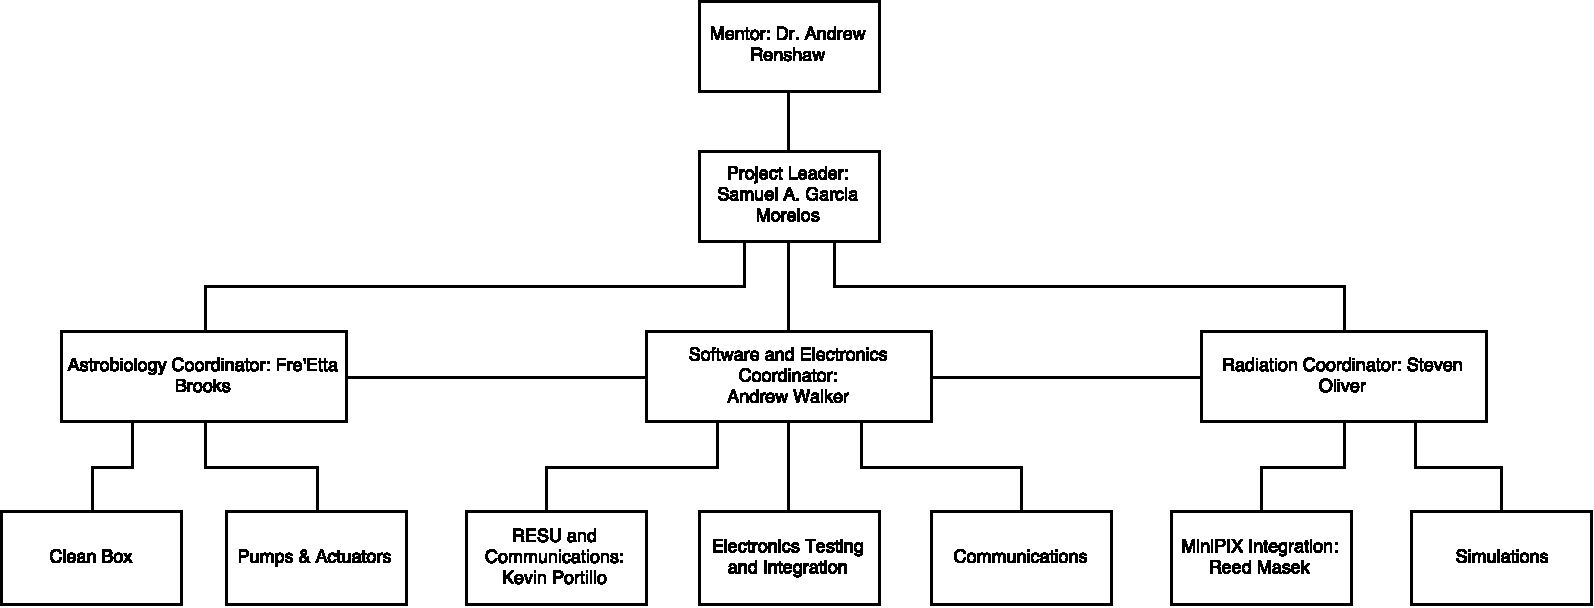
\includegraphics[width=1\textwidth]{./Figures/RoleTree.pdf}
\caption{Team role tree for the current SORA 2.0 UH team.}
\label{fig:role} 
\end{center}
\end{figure}

\subsection{Roles and Responsibilities}
\label{sec:Roles}
\begin{itemize}
\item PI – Dr. Andrew Renshaw
	\begin{itemize}
	\item Attend weekly team meetings and provide general research team guidance
	\item Review project design and final products for submission to HASP
	\item Attend monthly teleconferences.
	\item Equipment procurement
	\end{itemize}
\item Project Leader - Samuel A. Garcia Morelos
	\begin{itemize}
	\item Interface with HASP Flight Control Team and act as team main point of contact
	\item Compile monthly reports and submit to HASP
	\item Attend monthly teleconference with HASP
	\item Coordinate with PI on administration tasks and internal group business
	\item Coordinate meetings and assign tasks with deadlines
	\item Approve designs, tests, ideas, and any work related to HASP and payload
	\item Final decisions on staffing (Staffing decisions will be a group decision overall)
	\end{itemize}
\item Electronics and Communications Coordinator - Andrew Walker
	\begin{itemize}
	\item Do necessary reserach for finalizing work
	\item Coordinate information, tasks, and deadlines with subgroup
	\item Approve work done by subsystem team
	\item Write bimonthly updates along with detailed reports from subsytem meetings
	\item Make detailed presentations, if necessary, for weekly team meetings
	\item Report to project leader and PI with any project changes, issues encountered, and any external communications.
	\item CC PI and Project Leader in all emails for external communications
	\item Perform other such duties as the Project Leader or PI may specify
	\end{itemize}
\item Astrobiology Coordinator - Fre'Etta Brooks
	\begin{itemize}
	\item Do necessary reserach for finalizing work
	\item Coordinate information, tasks, and deadlines with subgroup
	\item Approve work done by subsystem team
	\item Write bimonthly updates along with detailed reports from subsytem meetings
	\item Make detailed presentations, if necessary, for weekly team meetings
	\item Report to project leader and PI with any project changes, issues encountered, and any external communications.
	\item CC PI and Project Leader in all emails for external communications
	\item Perform other such duties as the Project Leader or PI may specify
	\end{itemize}
\item Radiation Coordinator - Steven Oliver
	\begin{itemize}
	\item Do necessary reserach for finalizing work
	\item Coordinate information, tasks, and deadlines with subgroup
	\item Approve work done by subsystem team
	\item Write bimonthly updates along with detailed reports from subsytem meetings
	\item Make detailed presentations, if necessary, for weekly team meetings
	\item Report to project leader and PI with any project changes, issues encountered, and any external communications.
	\item CC PI and Project Leader in all emails for external communications
	\item Perform other such duties as the Project Leader or PI may specify
	\end{itemize}
\item RESU Lead Programmer - Kevin Portillo
	\begin{itemize}
	\item Do necessary reserach for finalizing work
	\item Coordinate with team
	\item Make detailed presentations, if necessary, for weekly team meetings
	\item Report to project leader and PI with any project changes, issues encountered, and any external communications.
	\item CC PI and Project Leader in all emails for external communications
	\item Perform other such duties as the Project Leader or PI may specify
	\end{itemize}
\item MiniPIX Integration and Testing - Reed Masek
	\begin{itemize}
	\item Do necessary reserach for finalizing work
	\item Coordinate with team and subsystem coordinator	
	\item Make detailed presentations, if necessary, for weekly team meetings
	\item Report to project leader and PI with any project changes, issues encountered, and any external communications.
	\item CC PI and Project Leader in all emails for external communications
	\item Perform other such duties as the Project Leader or PI may specify
	\end{itemize}
\item Team Member
	\begin{itemize}
	\item Do necessary reserach for finalizing work
	\item Coordinate with team and subsystem coordinator
	\item Make detailed presentations, if necessary, for weekly team meetings
	\item Report to project leader and PI with any project changes, issues encountered, and any external communications.
	\item CC PI and Project Leader in all emails for external communications
	\item Perform other such duties as the Project Leader or PI may specify
	\end{itemize}
\end{itemize}
		 
\subsection{Timeline}
\label{sec:Timeline}

% Please add the following required packages to your document preamble:
% \usepackage{graphicx}
\begin{table}[!h]
\centering
\caption{Timeline for the 2018 SORA 2.0 Mission}
\label{timeline}
\resizebox{\textwidth}{!}{%
\begin{tabular}{|c|l|}
\hline
\textbf{Month of 2018} & \multicolumn{1}{c|}{\textbf{Description of Work}} \\ \hline
\textbf{January} & \begin{tabular}[c]{@{}l@{}} * Secure funding \\ * Create and finish budget for mission \\ * Make inventory of hardware \\ * Procure hardware/software \\ * Start designs of SORA 2.0 \\ * Update RESU \\ * Upgrade vacuum chamber \\ * Recruit new members \end{tabular} \\ \hline
\textbf{February} & \begin{tabular}[c]{@{}l@{}}
* Continue with work from January.  Funding must be secured by end of March.\\ * Have finished list of inventory\\ * Finalize upgrades to vacuum chamber\\ * Continue recruitment and finalize by end of month.\\ * Continue design work of SORA 2.0\\ * Finish RESU upgrade\end{tabular} \\ \hline
\textbf{March} & \begin{tabular}[c]{@{}l@{}}Obtain funding by the end of this month.  Finish all tasks from the previous two months and transition into building phase.\\ * Have all hardware/software orders in by the end of the month\\ * Begin PSIP, have draft by end of the month\end{tabular} \\ \hline
\textbf{April} & \begin{tabular}[c]{@{}l@{}}* Order remaining items if needed\\ * Finish PSIP by April 25th\\ * RESU and MiniPIX integration and testing\\ * Upgrade clean room and prepare for astrobiology work\end{tabular} \\ \hline
\textbf{May} & \begin{tabular}[c]{@{}l@{}}* PSIP and FLOP development\\ * Finalize integration of RESU and hardware\\ * Continue working on astrobiology upgrades\end{tabular} \\ \hline
\textbf{June} & \begin{tabular}[c]{@{}l@{}}Final PSIP due June 27th\\ *Finalize astrobiology upgrades and ready for integration\\ * Testing in lab\end{tabular} \\ \hline
\textbf{July} & \begin{tabular}[c]{@{}l@{}}Final FLOP due July 31st\\ * Make changes from testing and continue tests\end{tabular} \\ \hline
\textbf{August} & \begin{tabular}[c]{@{}l@{}}Payload Integration (August 4 - 8)\\ *Have all payload work done and ready for flight\end{tabular} \\ \hline
\textbf{September} & * Launch and recovery TBA \\ \hline
\textbf{October} & Debrief and analyze all data from flight \\ \hline
\textbf{November} & Have final report by end of November \\ \hline
\textbf{December} & Final Report due on the 8th \\ \hline
\end{tabular}%
}
\end{table}

\subsection{Funding}
\label{sec:Funding}
Funding source TBA - Applying for funding throught the Physics Department - University of Houston

		
		
%\begin{figure}[!htb]
%\begin{center}
%
\includegraphics[width=0.5\textwidth]{./Figures/Test.jpg}
%\caption{This is a test figure.
%}
%\label{fig:Test} 
%\end{center}
%\end{figure}

	%Includes the following:
		%Team Structure
		%Timeline
		%Funding
	
%References
\newpage
%\section{References}
%\label{sec:References}

\begin{thebibliography}{9}
\bibitem{SORA}
S.A. Garcia Morelos, F.Brooks, S.Oliver, A.Walker, K.D. Portillo, R.B. Masek, D.Mroczek, D.Pena, J.Juarez, A.Cruz, D. Henandez, S.George, D. Pattison, A.L.Renshaw. \textit{Scientific Report for the UH Team.} SORA 2017 Mission Webpage. \url{http://laspace.lsu.edu/hasp/groups/Payload.php?py=2017&pn=10}.

\bibitem{silicon_sensor}
  MiniPIX - Miniaturized Portable USB Photon Counting Camera. (n.d.). Retrieved February 02, 2017, from \url{http://advacam.com/camera/minipix}.

\bibitem{LSU}
  Christner, B., Alleman, M., Bryan, N., Burke, S., Guzik, T.G., Granger, D., King, G. (2013) \textit{LSU HASP2013 PDF. Baton Rouge: Louisiana Space Consortium}.

%\bibitem{SolidWorks}
%  SolidWorks 3D CAD software \url{http://www.solidworks.com/}.

\bibitem{Extremophiles}
  Extremophiles \href{http://www.nytimes.com/2013/02/07/science/living-bacteria-found-deep-under-antarctic-ice-scientists-say.html}{http://www.nytimes.com/2013/02/07/science/living-bacteria-found-deep-\\under-antarctic-ice-scientists-say.html}.

\bibitem{canales}
 Canales D. C. and Ehteshami A., \textit{An attempt to sample atmospheric bacteria}, Houston, TX, 2015, January 11.

\bibitem{bexus}
Urbar, J., Scheirich, J., Jakubek, J., 2011. Medipix/Timepix cosmic ray tracking on BEXUS stratospheric balloonflights. Nucl. Instrum. Methods A 633, S206-209.
	
%\bibitem{uv_irradiance}
%  Calculating the UV Index. (2016, October 14). Retrieved June 03, 2017, from \url{https://www.epa.gov/sunsafety/calculating-uv-index-0}.

%\bibitem{cleanbox}
% Clean box material \url{https://www.mcmaster.com/\#uhmw-polyethylene/=1aijn1p}.

%\bibitem{valve}
% Valve data sheet \url{http://www.generant.com/Literature/Series\%20VRV\%20Product\%20Literature.pdf}.

\bibitem{advacam}
  ADVACAM at \url{advacam.com}.

\bibitem{medipix}
  Medipix collaboration at \url{https://medipix.web.cern.ch/}.
  
\bibitem{stuartthesis} 22
  George, S., \textit{Dosimetric Applications of Hybrid Pixel Detectors}, University of Wollongong, Australia, 2015.

%\bibitem{mpdatasheet}
%  ADVACAM, \textit{MINIPIX Version 1.0 Datasheet}, Retrieved from \url{http://www.widepix.cz/files/datasheets/MiniPIX\%20v1.0\%20Datasheet.pdf}.

%\bibitem{mpjakubek}
%  Jan Jakubek, \textit{Precise energy calibration of pixel detector working in time-over-threshold mode} Institute of Experimental and Applied Physics, Czech Technical University in Prague, Czech Republic, 2011.
  

    


%\bibitem{magnetictool}
%  United States National Oceanic and Atmospheric Administration, \textit{Magnetic Field Calculators} [Data sets], Retrieved from \url{https://www.ngdc.noaa.gov/geomag-web/#igrfwmm}.

%\bibitem{gorman}
%	Gorman, J. (2013, February 06). \textit{Scientists Find Life in the Cold and Dark Under Antarctic Ice.} Retrieved September 15, 2016, from Scientists Find Life in the Cold and Dark Under Antarctic Ice.
	
 
 
%\bibitem{pumpsource}
%  \url{http://www.knfusa.com/?type=5600&amp;file=2079}.


%\bibitem{Horneck}
%  Horneck, G. 1993. The Biostack concept and its application in space and at accelerators: studies in Bacillus subtilis spores, p. 99-115. In C. E. Swenberg, G. Horneck, and E. G. Stassinopoulos (ed.), \textit{Biological effects and physics of solar and galactic cosmic radiation}[PDF], part A. Plenum Press, New York, NY. accessed 10/24/16  

%\bibitem{Horneck} 
%  Horneck, G. 2007. \textit{Space radiation biology}[PDF], p. 243-273. In E. Brinckmann (ed.), Biology in space and life on Earth. Wiley-VCH, Weinheim, Germany. Accessed 10/26/16

%\bibitem{Horneck}
%  Horneck, G., C. Baumstark-Khan, and G. Reitz. 2002. \textit{ Space microbiology: effects of ionizing radiation on microorganisms in space}[PDF], p. 2988-2996. In G. Bitton (ed.), The encyclopedia of environmental microbiology. John Wiley \& Sons, New York, NY. Accessed 10/30/16

%\bibitem{Horneck}
%  Horneck, G., C. Baumstark-Khan, and R. Facius. 2006. \textit{Radiation biology}[PDF], p. 292-335. In G. Cl?ment and K. Slenzka (ed.), Fundamentals of space biology. Kluwer Academic Publishers/Springer, Dordrecht, The Netherlands. accessed 11/4/16

%\bibitem{Kiefer}
%Kiefer, J., K. Schenk-Meuser, and M. Kost. 1996. \textit{Radiation biology}[PDF], p. 300-367. In D. Moore, P. Bie, and H. Oser (ed.), Biological and medical research in space. Springer, Berlin, Germany. accessed 11/9/16
 
	

\bibitem{SamURD}
	Alfonso Garcia Morelos, S. (2016, October 13).
	\textit{A Novel Microbe Trap.}
	Presentation at UH Undergraduate Research Day. \url{http://www.uh.edu/honors/undergraduate-research/}
	
	
%\bibitem{StevenURD}

%\bibitem{FreEttaWomensConference}

%\bibitem{StevenSchoolPres}

%\bibitem{StevenURD}
%  Oliver, S. J. (2017, October 12). 
%  \textit{Stratospheric Organism and Radiation Analyzer}
%  Presentation at UH Undergraduate Research Day. Retrieved October 12, 2017, from \url{http://www.uh.edu/honors/undergraduate-research/events/urday2017/}

%\bibitem{StevenSchoolPres}
%  Oliver, S. J. (2017, November 4). 
%  \textit{STEM Life at UH}
%  Presentation at UH Gathering of the Eagles STEM Symposium. \url{https://www.uh.edu/news-events/stories/2016/November/110416EaglesSTEM.php}

%\bibitem{Fre}
%  Brooks, F. (2017, January 14).
%  \textit{Stratospheric Organism and Radiation Analyzer}
%  Presentation at Rice University, APS Conferences for Undergraduate Women in Physics (CUiP). \url{http://www.google.com/url?q=http%3A%2F%2Fwww.aps.org%2Fprograms%2Fwomen%2Fworkshops%2Fcuwip.cfm&sa=D&sntz=1&usg=AFQjCNE5pImV-SVrb87CvgAa9RSfeCrYXg}  
  
%\bibitem{SamAPS}
%	Alfonso Garcia Morelos, S. (2017, October 20).
%	\textit{Stratospheric Organism and Radiation Analyzer}
%	Retrieved October 20, 2017, from \textit{Bulletin of the American Physical Society}. \url{https://meetings.aps.org/Meeting/TSF17/Session/E5.3}
	
  
%  \bibitem{MIT}
%	MIT-Lemelson Award 2018.
%	\url{https://lemelson.mit.edu/}
  

\end{thebibliography}
%Bibliography file

%---------------------------------------------DO NOT USE IN APPLICATION---------------
%Results and Analysis
%Section: Flight Conditions and Environmental Data
%\input{Results.tex} %RESU first
%\input{Results_Rad.tex} %MiniPIX last
%\newpage
%\input{Results_Astro.tex} %Astro second

%\input{Results_UV.tex}
%\input{Simulations.tex} %Simulations results

%Discussion
%\input{Discussion_RESU.tex} %RESU first
%\input{Discussion_Astro.tex} %Astro second
%\input{Discussion_Rad.tex} %MiniPIX last
%\input{Discussion_Simulations.tex} %Simulations discussion

%Conclusion
%\input{Conclusion.tex} 
%\newpage
%Appendix
%\input{Appendix.tex}
%\newpage

%
%\clearpage
%\bibliographystyle{SORA}
%\bibliography{SORA}
\end{document}
